\documentclass[10pt,twocolumn,letterpaper]{article}

\usepackage[top=0.75in,bottom=0.75in,left=0.65in,right=0.65in,columnsep=0.2in]{geometry}
\usepackage{graphicx}
\usepackage{booktabs}
\usepackage{array}
\usepackage{tabularx}
\usepackage{hyperref}
\usepackage{xcolor}
\usepackage{amsmath}
\usepackage[T1]{fontenc}
\usepackage{lmodern}

\definecolor{accent}{HTML}{0F172A}
\definecolor{muted}{HTML}{64748B}
\definecolor{rule}{HTML}{CBD5E1}

\hypersetup{colorlinks=true,linkcolor=accent,urlcolor=muted,citecolor=muted,
  pdftitle={Vaartha: Geopolitical Supply Chain Intelligence}}

\setlength{\parskip}{3pt}
\setlength{\parindent}{0pt}
\setlength{\abovecaptionskip}{4pt}
\setlength{\belowcaptionskip}{2pt}
\setlength{\intextsep}{6pt}
\setlength{\textfloatsep}{6pt}

% Compact section headings
\makeatletter
\renewcommand\section{\@startsection{section}{1}{\z@}%
  {-6pt \@plus -2pt \@minus -1pt}{3pt \@plus 1pt}%
  {\normalfont\normalsize\bfseries\color{accent}}}
\renewcommand\subsection{\@startsection{subsection}{2}{\z@}%
  {-4pt \@plus -1pt \@minus -1pt}{2pt \@plus 1pt}%
  {\normalfont\small\bfseries\color{accent}}}
\makeatother

% Compact figure captions
\makeatletter
\long\def\@makecaption#1#2{%
  \vskip\abovecaptionskip
  {\small\textbf{#1.} #2\par}
  \vskip\belowcaptionskip}
\makeatother

\pagestyle{plain}

% ══════════════════════════════════════════════════════════════════════════════
\begin{document}

% ── Title (single column) ─────────────────────────────────────────────────────
\twocolumn[{%
\begin{center}
{\large\bfseries\color{accent}
  Vaartha: Geopolitical Supply Chain Intelligence\\[0.3em]
  {\normalsize\mdseries\color{muted}
    Escalating Geopolitical Fragmentation, Critical Mineral Supply Chains,\\
    and Corporate Capital Allocation --- A Linked Exploratory Analysis}}\\[0.6em]
{\small
  \textbf{Team 7 Lambda} $\cdot$ Rutgers University $\cdot$ Advanced Python SP2026
  \quad|\quad
  Tarun Theegela (tt633) $\cdot$ Sai Raunak Bidesi (ssb196) $\cdot$
  Chaitanya Deogaonkar (cmd517) $\cdot$ Satwik Nadipelli (srn91)
}\\[0.5em]
\noindent\textcolor{rule}{\rule{\linewidth}{0.5pt}}\\[0.5em]
\end{center}
\begin{center}
\parbox{0.92\linewidth}{\small\itshape
\textbf{Abstract.}
This report examines how escalating geopolitical fragmentation distorts global supply chains for
critical minerals and forces corporations to restructure capital expenditure. Using 13 years of
data (2010--2022) across four linked subtopics---critical mineral supply concentration (ST1),
geopolitical risk transmission (ST2), national energy policy divergence (ST3), and corporate
CapEx behavior (ST4)---we trace a causal chain from geopolitical shock to investment response.
Key findings: gallium and germanium are near-monopolies (HHI\,$>$\,0.75); geopolitical risk leads
supply chain pressure by 1--2 months; policy divergence is accelerating asymmetric mineral demand;
and semiconductor firms increase capital intensity within 1--2 years of a GPR spike.
All analysis is strictly exploratory and descriptive; no inferential statistics are used.
}
\end{center}
\vspace{0.5em}
\noindent\textcolor{rule}{\rule{\linewidth}{0.5pt}}\\[0.6em]
}]

% ══════════════════════════════════════════════════════════════════════════════
\section{Introduction and Thesis}

The global economy depends on a small set of minerals---lithium, cobalt, gallium, germanium,
rare earths, copper, nickel---that are geographically concentrated and indispensable for
semiconductors, EV batteries, and solar panels. When geopolitical relationships between producer
and consumer nations deteriorate, the consequences reach corporate balance sheets.

\textbf{Thesis:} \textit{Escalating geopolitical fragmentation systematically distorts global
supply chains of critical energy-transition and AI-hardware minerals, forcing technology and
energy conglomerates to aggressively restructure CapEx and R\&D to achieve decoupled
profitability and risk resilience.}

We organize this as a four-step causal chain:
\begin{center}
\small
ST2 $\!\rightarrow\!$ ST1 $\!\rightarrow\!$ ST3 $\!\rightarrow\!$ ST4
\\[0.2em]
\textit{Geopolit. Risk $\to$ Supply Distortion $\to$ Policy Amplification $\to$ CapEx Response}
\end{center}

Each step is supported by an independent dataset and exploratory visualization. All findings are
descriptive; causal language is a framing device only.

% ══════════════════════════════════════════════════════════════════════════════
\section{Data and Methodology}

\begin{table}[htbp]
\centering
\caption{Datasets across all four subtopics.}
\label{tab:data}
\scriptsize
\setlength{\tabcolsep}{3pt}
\begin{tabular}{llp{2.2cm}l}
\toprule
\textbf{ST} & \textbf{Dataset} & \textbf{Source} & \textbf{Coverage} \\
\midrule
ST1 & BGS Mineral Stats    & British Geol.\ Survey    & 2010--22, 11 min. \\
ST1 & World Bank Pink Sheet & World Bank              & 2010--22, monthly \\
ST1 & OECD Export Restrict. & OECD                   & 2010--22          \\
ST2 & GPR Index             & Iacoviello (2022)       & 2010--22, monthly \\
ST2 & NY Fed GSCPI          & Fed.\ Reserve N.Y.      & 2010--22, monthly \\
ST2 & FRED + Sector ETFs    & St.\ Louis Fed / Yahoo  & 2010--22, monthly \\
ST3 & OWID Energy           & Our World in Data       & 2010--22, annual  \\
ST3 & RFF Carbon Pricing    & Resources for Future    & 2010--20, annual  \\
ST4 & SEC EDGAR XBRL        & U.S.\ SEC               & 2010--22, qtrly   \\
\bottomrule
\end{tabular}
\end{table}

The analysis window (2010--2022) is bounded by XBRL mandatory filing adoption (lower) and RFF
carbon pricing coverage (upper). The 2022 cutoff captures the Ukraine invasion, the CHIPS Act,
and the post-COVID supply chain crisis---the three most consequential events for the thesis.

\textbf{Methods:} HHI for supply concentration; rolling Pearson correlations for co-movement;
OLS via \texttt{numpy.linalg.lstsq} for descriptive magnitudes only. All time-series joins use
\texttt{pd.merge\_asof(direction=`backward')} to prevent look-ahead bias.

% ══════════════════════════════════════════════════════════════════════════════
\section{ST1 --- Critical Mineral Chokepoints}

Critical mineral production is not merely concentrated---it has been monopolistic in several
categories for over a decade with no structural improvement. Gallium (HHI\,$\approx$\,0.77) and
germanium (HHI\,$\approx$\,0.76), both essential for semiconductor fabrication, are dominated by
China and have shown no diversification trend across the entire analysis window (Fig.\
\ref{fig:hhi_time}). Rare earths stand at HHI\,$\approx$\,0.71. A single geopolitical
deterioration with China simultaneously disrupts gallium, germanium, rare earths, and graphite
supply chains---a correlated shock, not an isolated one.

\begin{figure}[htbp]
\centering
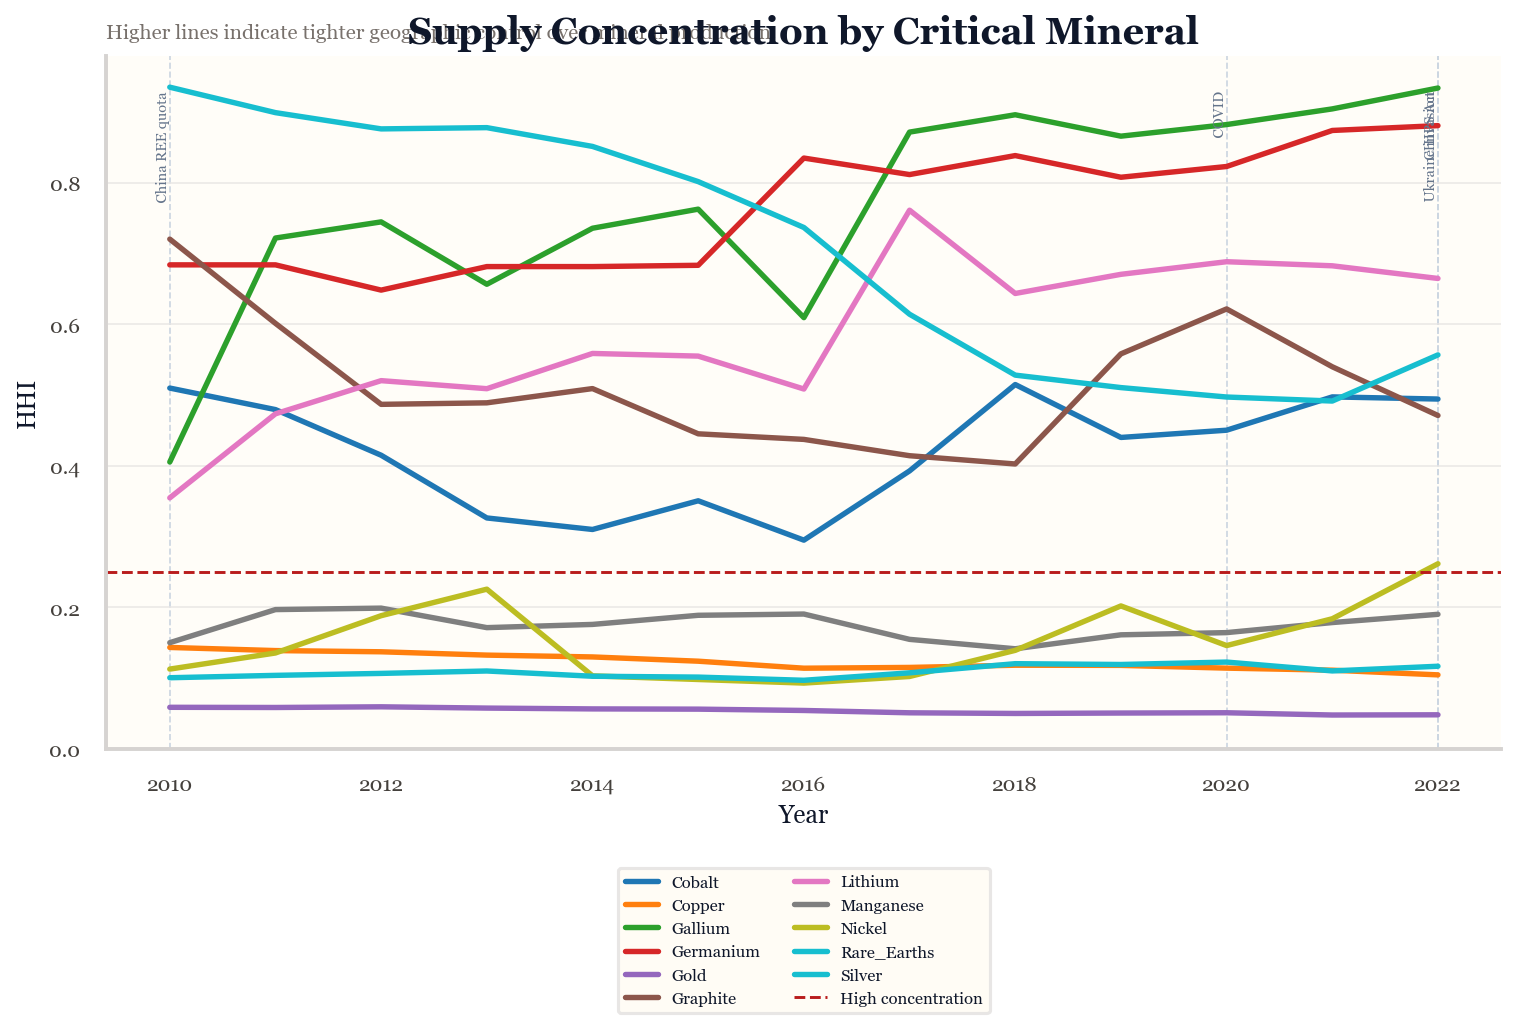
\includegraphics[width=\columnwidth]{outputs/charts/st1_hhi_over_time.png}
\caption{HHI by mineral, 2010--2022. Included to show that supply fragility is structural,
not cyclical: gallium, germanium, and rare earths have remained above the high-concentration
threshold (0.25, red dashed) for 13 years with no downward trend.}
\label{fig:hhi_time}
\end{figure}

Concentration translates into price volatility. The scatter in Fig.\ \ref{fig:hhi_vol} shows
that minerals with higher HHI exhibit greater 12-month rolling price volatility---supply chain
fragility is already priced into commodity markets.

\begin{figure}[htbp]
\centering
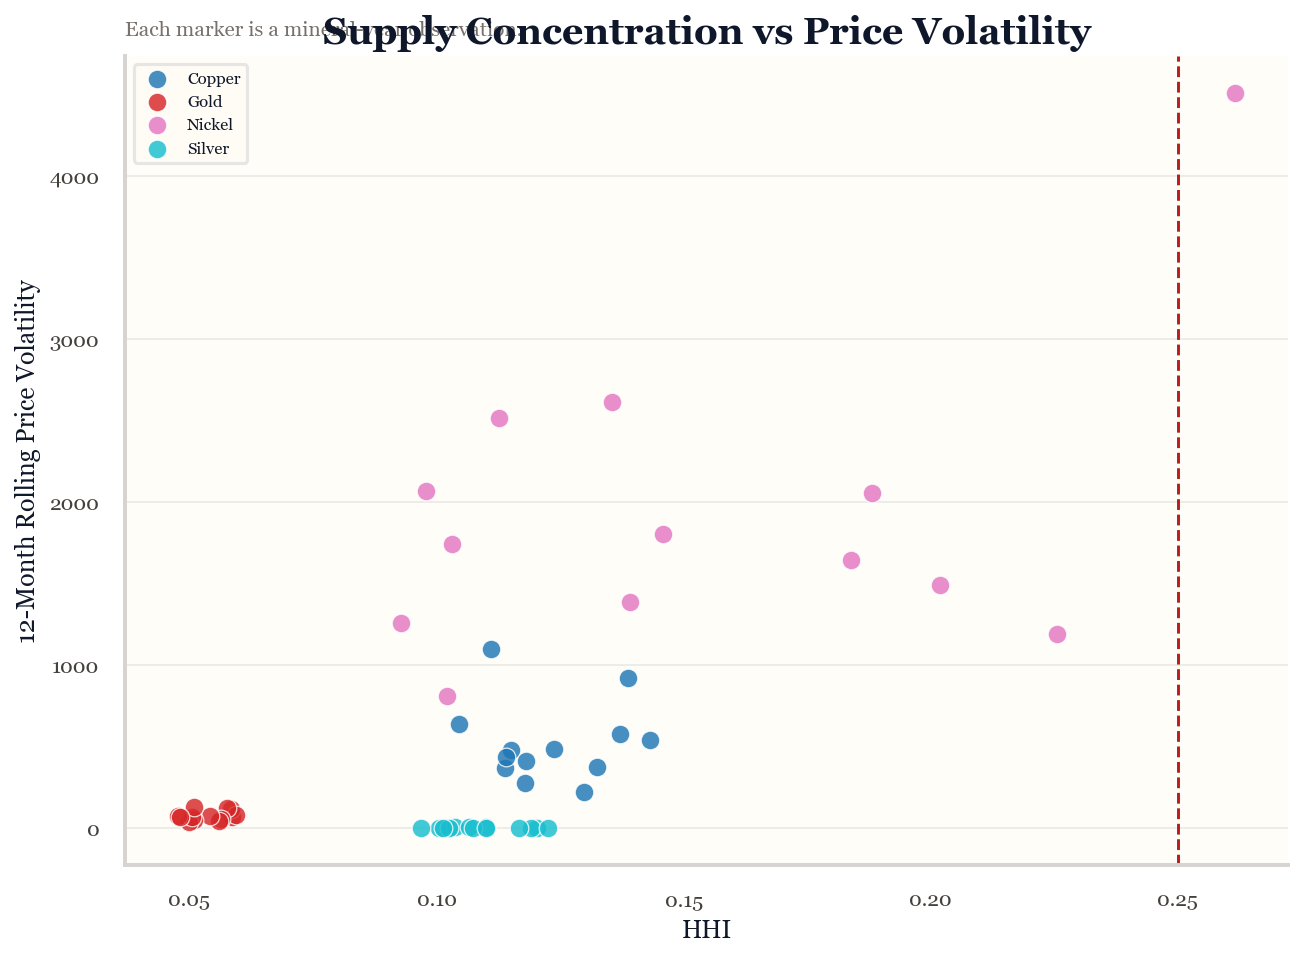
\includegraphics[width=\columnwidth]{outputs/charts/st1_hhi_vs_volatility.png}
\caption{HHI vs.\ 12-month rolling price volatility (mineral-year obs.). Included to
demonstrate that concentration is a financial risk, not just an abstract policy concern.}
\label{fig:hhi_vol}
\end{figure}

The policy response is accelerating the problem. OECD-tracked export restrictions on raw
materials nearly doubled between 2015 and 2022 (Fig.\ \ref{fig:oecd}), spiking after the
Ukraine invasion. Export restrictions are the mechanism through which geopolitical actors
(ST2) directly activate supply chain disruption (ST1).

\begin{figure}[htbp]
\centering
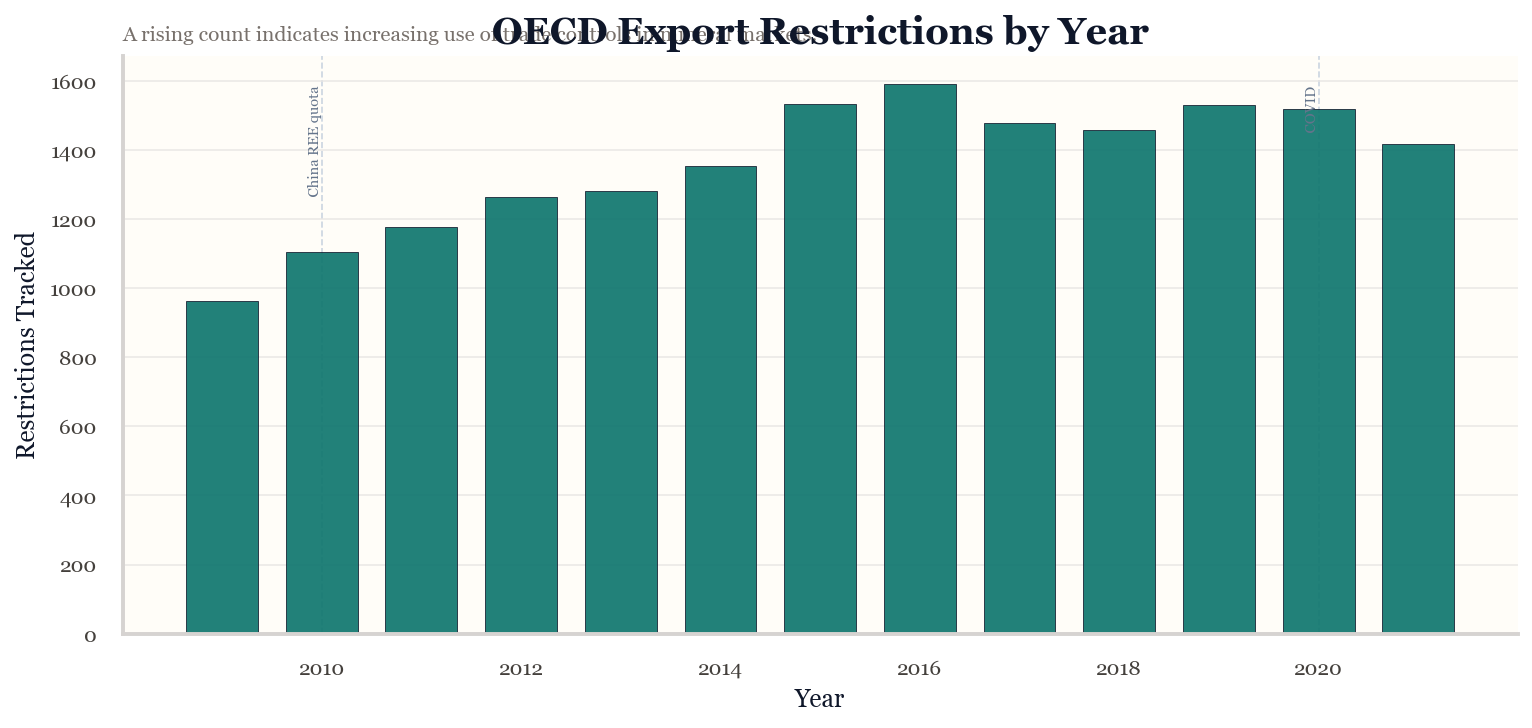
\includegraphics[width=\columnwidth]{outputs/charts/st1_oecd_restrictions.png}
\caption{OECD export restrictions by year. Included because rising restriction counts are the
empirical bridge between geopolitical intent (ST2) and supply chain disruption (ST1)---policy
translating risk into reality.}
\label{fig:oecd}
\end{figure}

\textit{Two supplementary interactive figures (production choropleth and trade-flow Sankey)
are provided as HTML files in \texttt{outputs/charts/}.}

% ══════════════════════════════════════════════════════════════════════════════
\section{ST2 --- Geopolitical Risk Transmission}

The Iacoviello GPR Index, constructed from newspaper counts of geopolitical tension language,
disaggregates into GPRT (threats: forward-looking) and GPRA (acts: realized events). GPRA spikes
are sharper and produce faster downstream price responses. Visible spikes in Fig.\
\ref{fig:gpr_ts} align precisely with Crimea (2014), the U.S.--China trade war (2018), COVID
(2020), and the Ukraine invasion (2022)---validating the index as a reliable signal.

\begin{figure}[htbp]
\centering
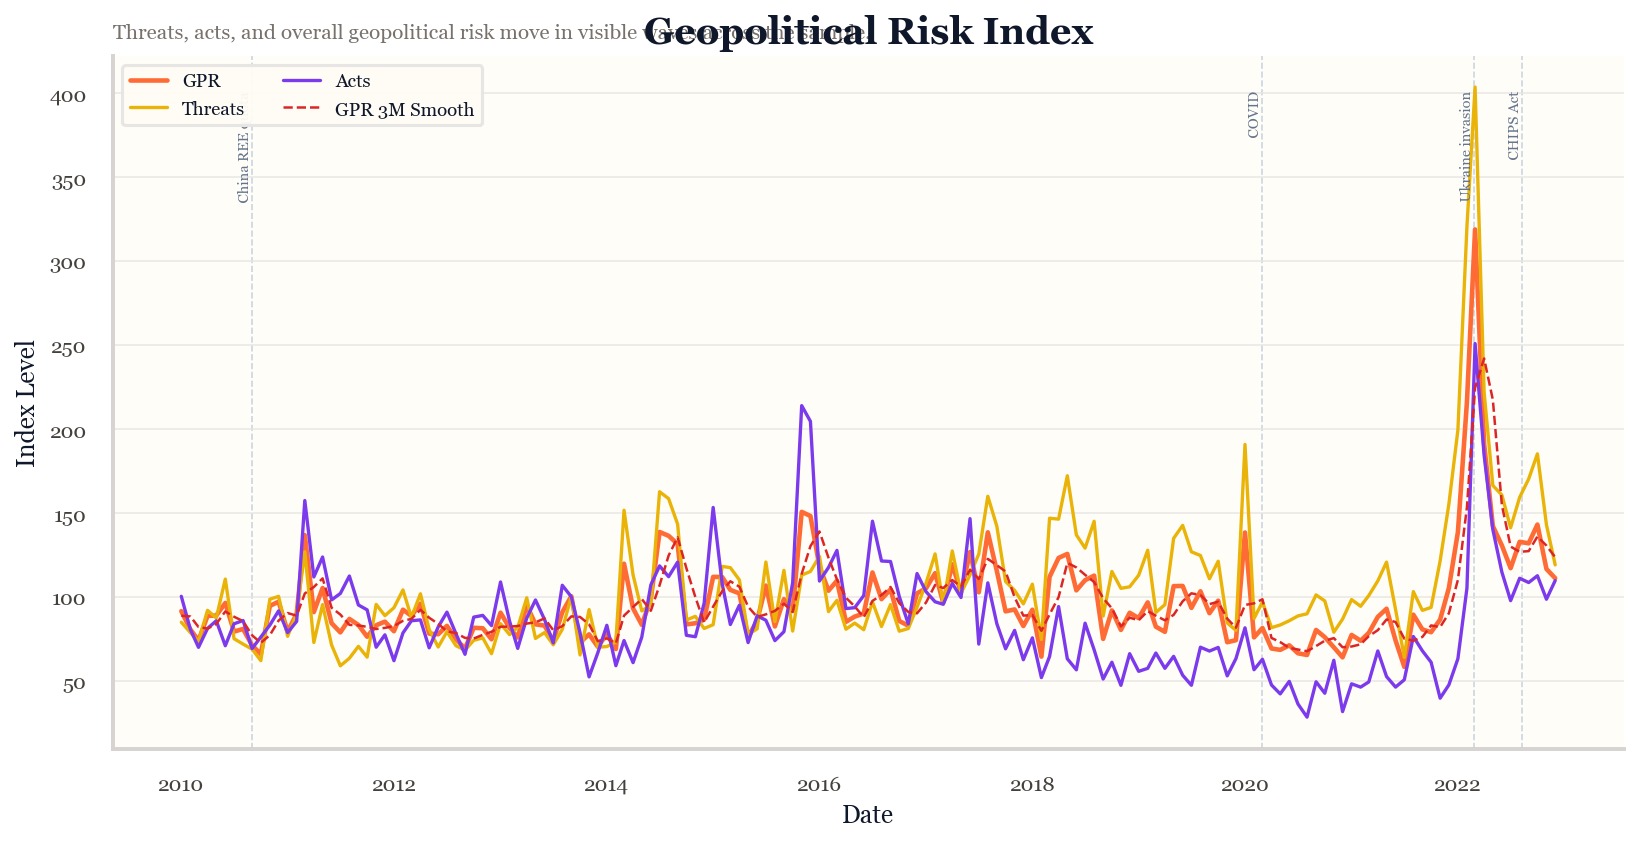
\includegraphics[width=\columnwidth]{outputs/charts/st2_gpr_timeseries.png}
\caption{GPR, GPRT, GPRA with 3-month smoothing. Included to establish that the index
captures real geopolitical episodes; each major spike corresponds to an identifiable event.}
\label{fig:gpr_ts}
\end{figure}

The key transmission finding is in Fig.\ \ref{fig:gpr_gscpi}: the 24-month rolling correlation
between GPR and GSCPI has been persistently positive since 2016 and strengthened materially
after 2020. This is not an artifact of a single event---it reflects a structural shift in which
geopolitical risk has become a more reliable predictor of supply chain pressure in the era of
great-power competition.

\begin{figure}[htbp]
\centering
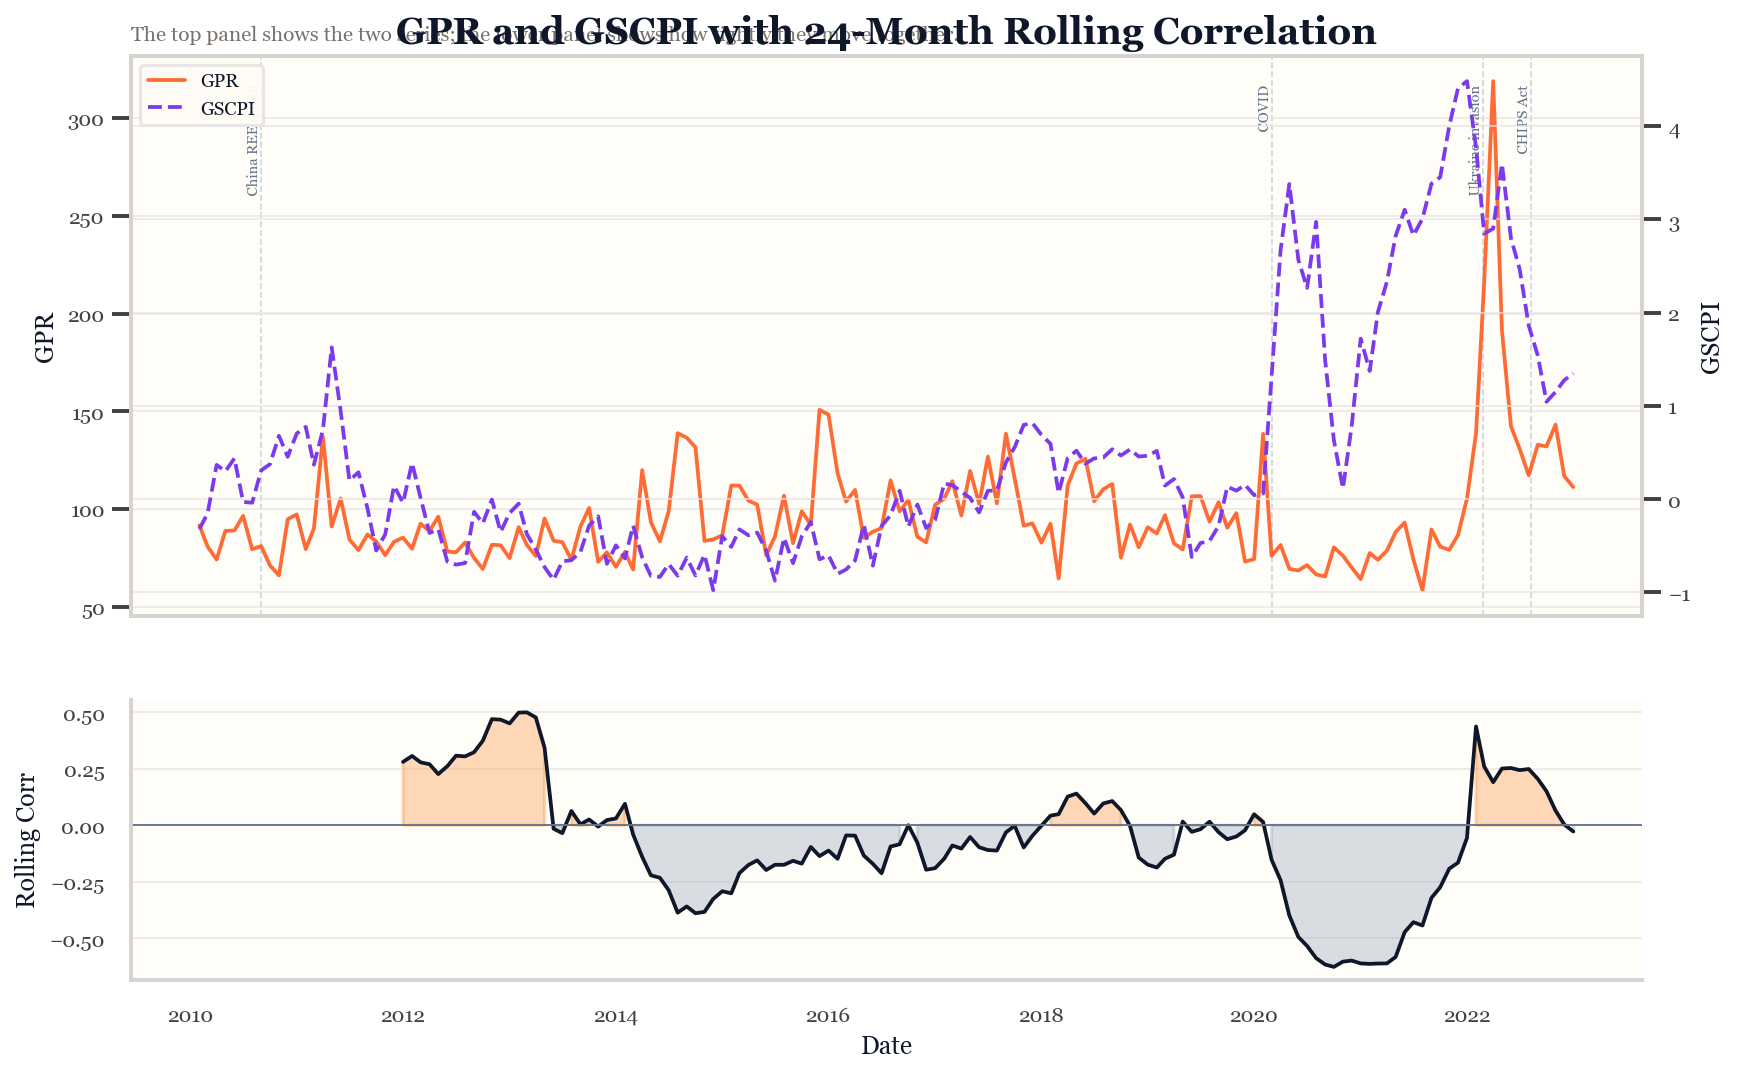
\includegraphics[width=0.98\columnwidth]{outputs/charts/st2_gpr_gscpi_correlation.png}
\caption{GPR and GSCPI with 24-month rolling correlation (lower panel). Included as the
foundational transmission proof: the positive rolling correlation has strengthened since 2016,
confirming that geopolitical risk systematically precedes supply chain disruption.}
\label{fig:gpr_gscpi}
\end{figure}

Supply chain pressure has asymmetric sectoral effects (Fig.\ \ref{fig:etf_corr}): it benefits
commodity producers (XLB positive correlation with GSCPI) while hurting technology consumers
(XLK, SOXX negative). This asymmetry is the behavioral mechanism that compels technology firms
to respond with CapEx restructuring---firms hurt by supply chain tightening must build
redundancy. The 2022 annual return heatmap (Fig.\ \ref{fig:etf_heat}) makes this visceral:
XLE $+65\%$, SOXX $-35\%$---a 100-point spread in a single year driven by geopolitical dynamics.

\begin{figure}[htbp]
\centering
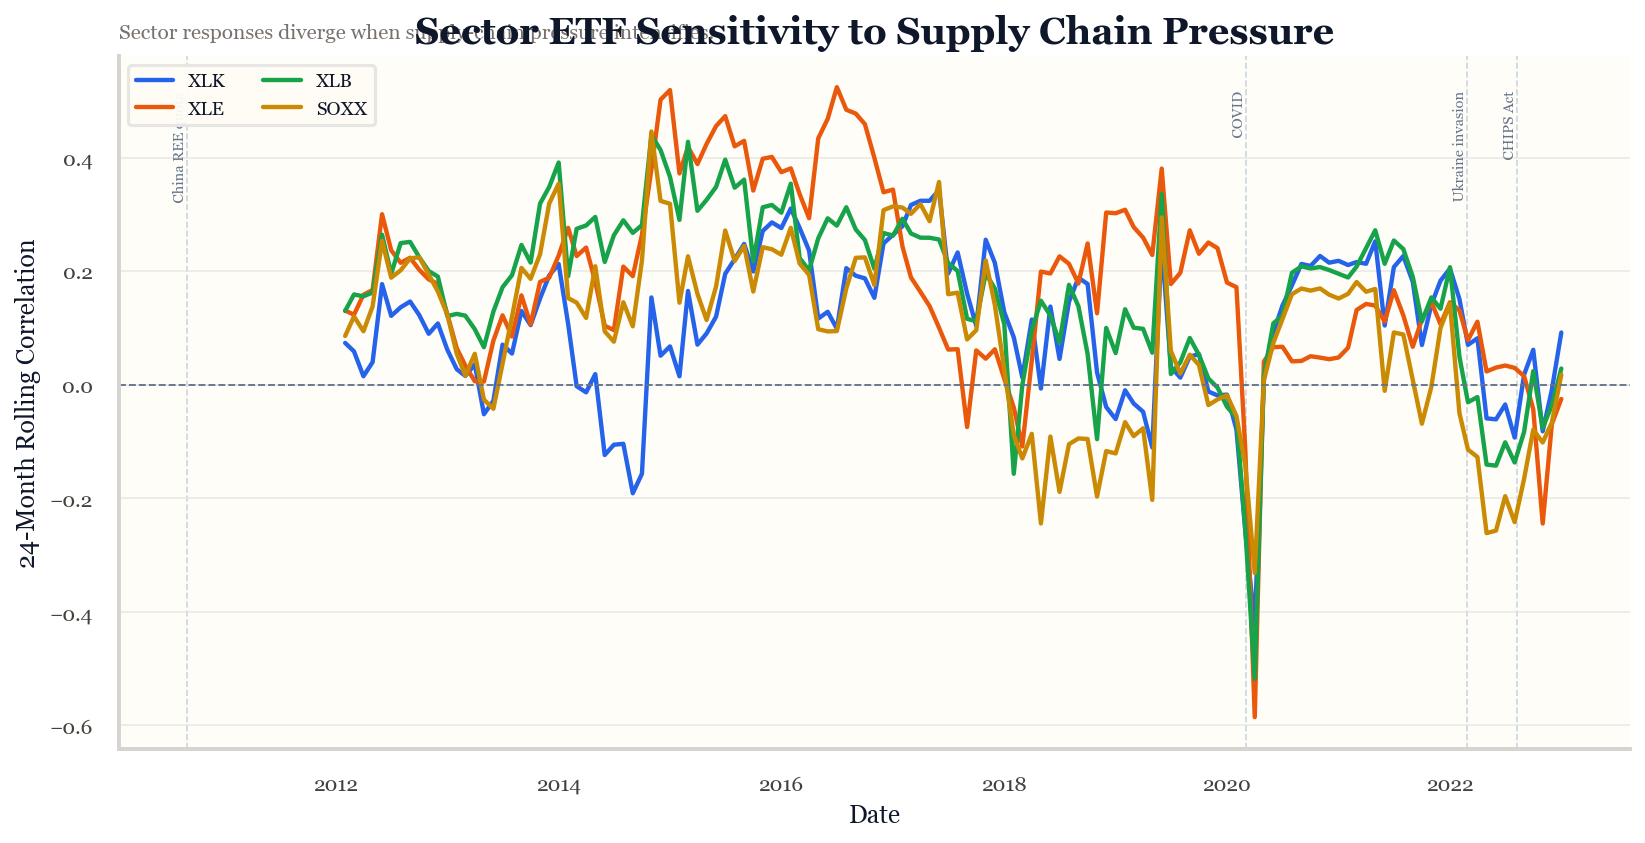
\includegraphics[width=\columnwidth]{outputs/charts/st2_gscpi_etf_correlation.png}
\caption{Sector ETF rolling correlation with GSCPI. Included to show the asymmetry that
drives the ST4 CapEx response: technology and semiconductor firms lose when supply chains
tighten, giving them incentive to build redundant capacity.}
\label{fig:etf_corr}
\end{figure}

\begin{figure}[htbp]
\centering
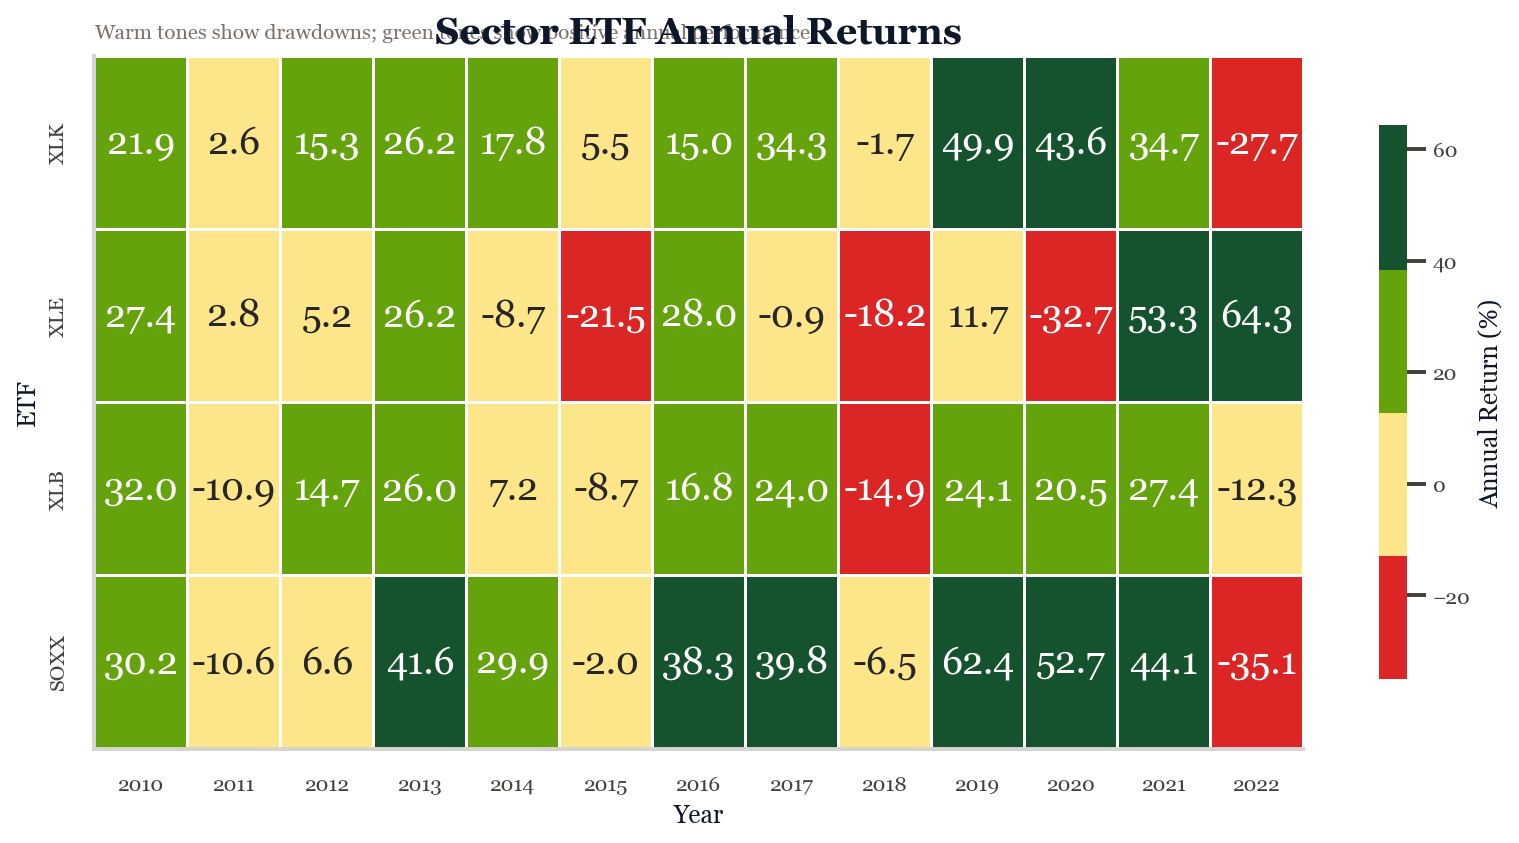
\includegraphics[width=\columnwidth]{outputs/charts/st2_etf_annual_heatmap.png}
\caption{Sector ETF annual returns heatmap. Included for the 2022 row alone: a 100-point spread
between energy and semiconductors is the clearest single-year quantification of geopolitical
supply chain impact on corporate equity value.}
\label{fig:etf_heat}
\end{figure}

The Ukraine event study (Fig.\ \ref{fig:ukraine}) provides a focused natural experiment: in a
$\pm$6-month window around February 24, 2022, GPR spikes immediately, GSCPI follows with a
1--2 month lag, and sector ETFs diverge sharply. The visual time-ordering is the most direct
descriptive evidence that the causal chain operates in the expected sequence.

\begin{figure}[htbp]
\centering
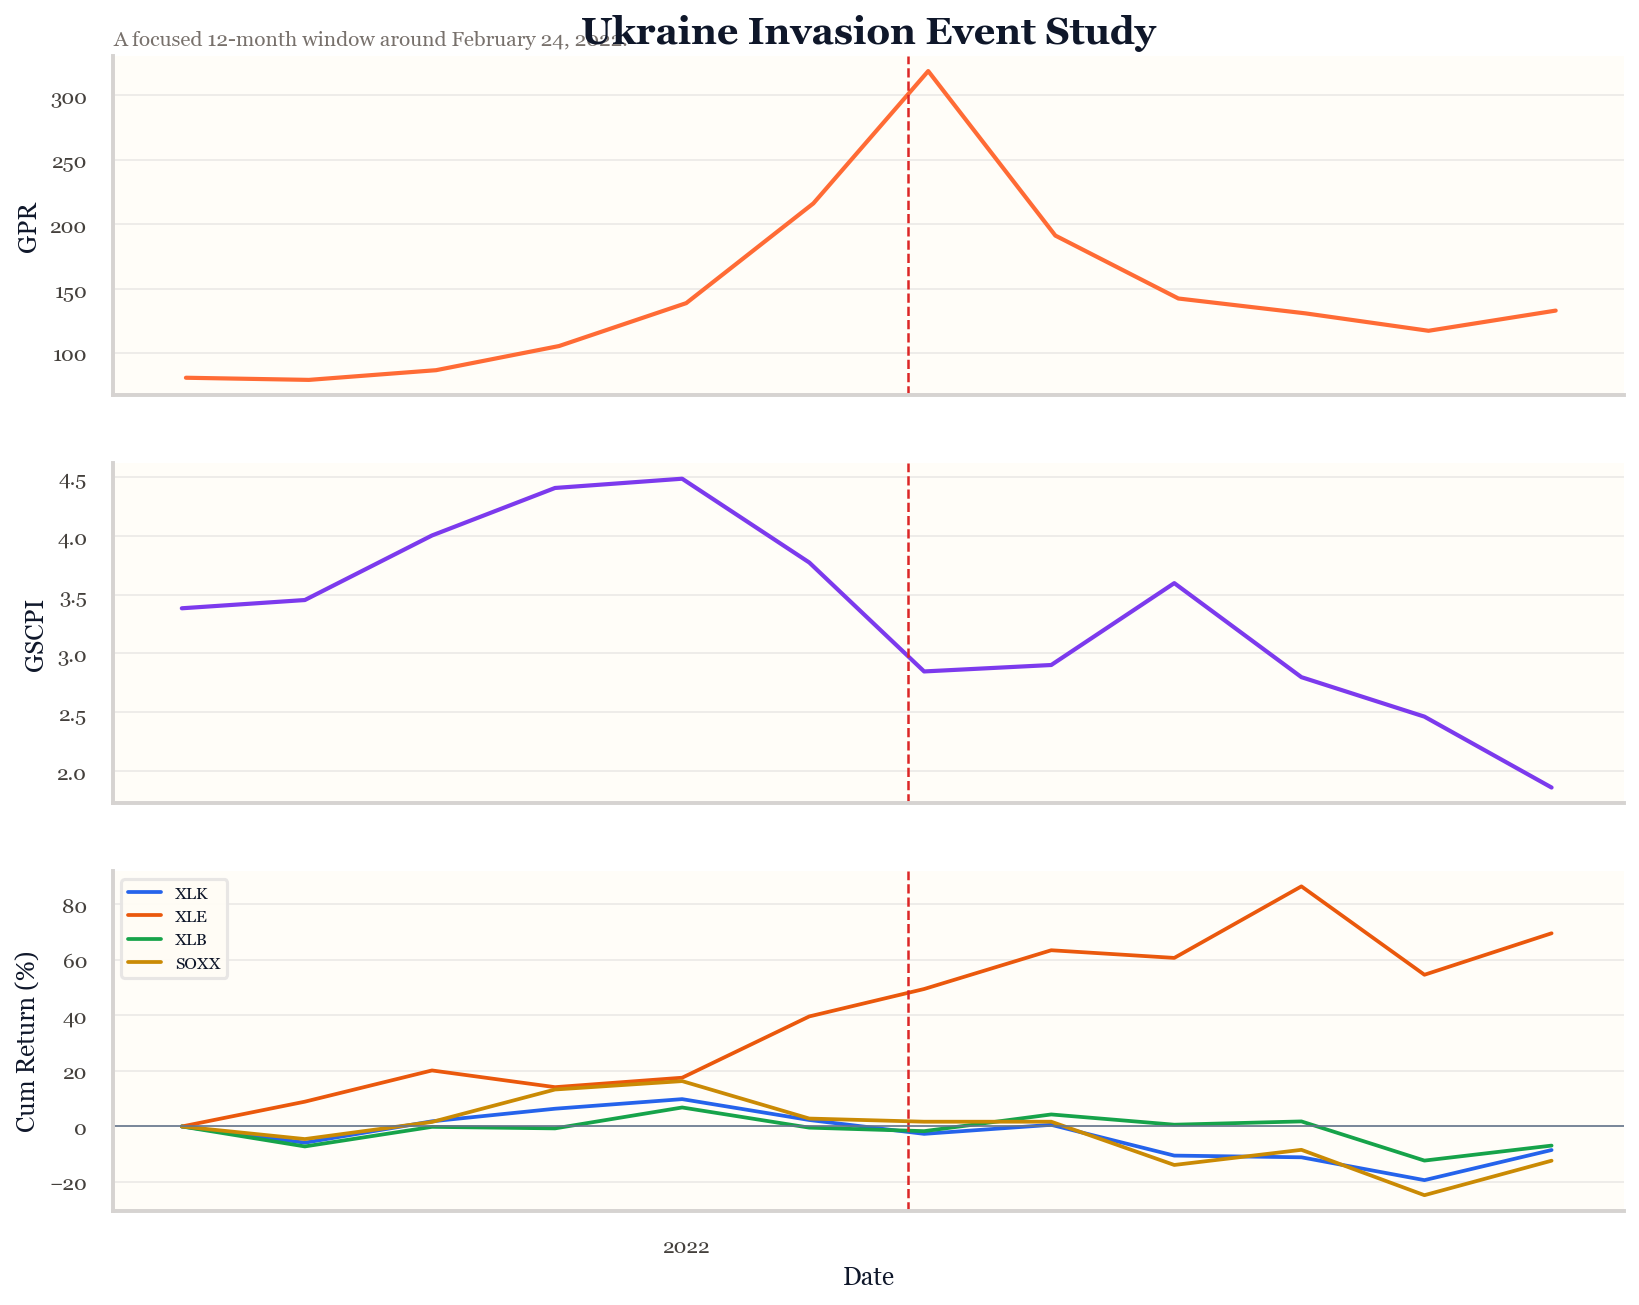
\includegraphics[width=0.98\columnwidth]{outputs/charts/st2_event_study_ukraine.png}
\caption{Ukraine invasion event study ($\pm$6 months). Included as a controlled natural
experiment: GPR spikes first (top), GSCPI follows with 1--2 month lag (middle), sector
ETFs diverge immediately (bottom). Time-ordering matches the proposed transmission mechanism.}
\label{fig:ukraine}
\end{figure}

% ══════════════════════════════════════════════════════════════════════════════
\section{ST3 --- Energy Policy Amplifies Mineral Demand}

Divergent national energy policies create structurally different mineral demand trajectories.
Germany and the UK have pursued steep renewables acceleration since 2015; India and Australia
remain predominantly fossil-fuel dependent (Fig.\ \ref{fig:energy_mix}). This divergence means
that demand for lithium, silicon, copper, and cobalt is growing at structurally different rates
across our focal countries---compounding pressure on the concentrated supply chains in ST1.

\begin{figure}[htbp]
\centering
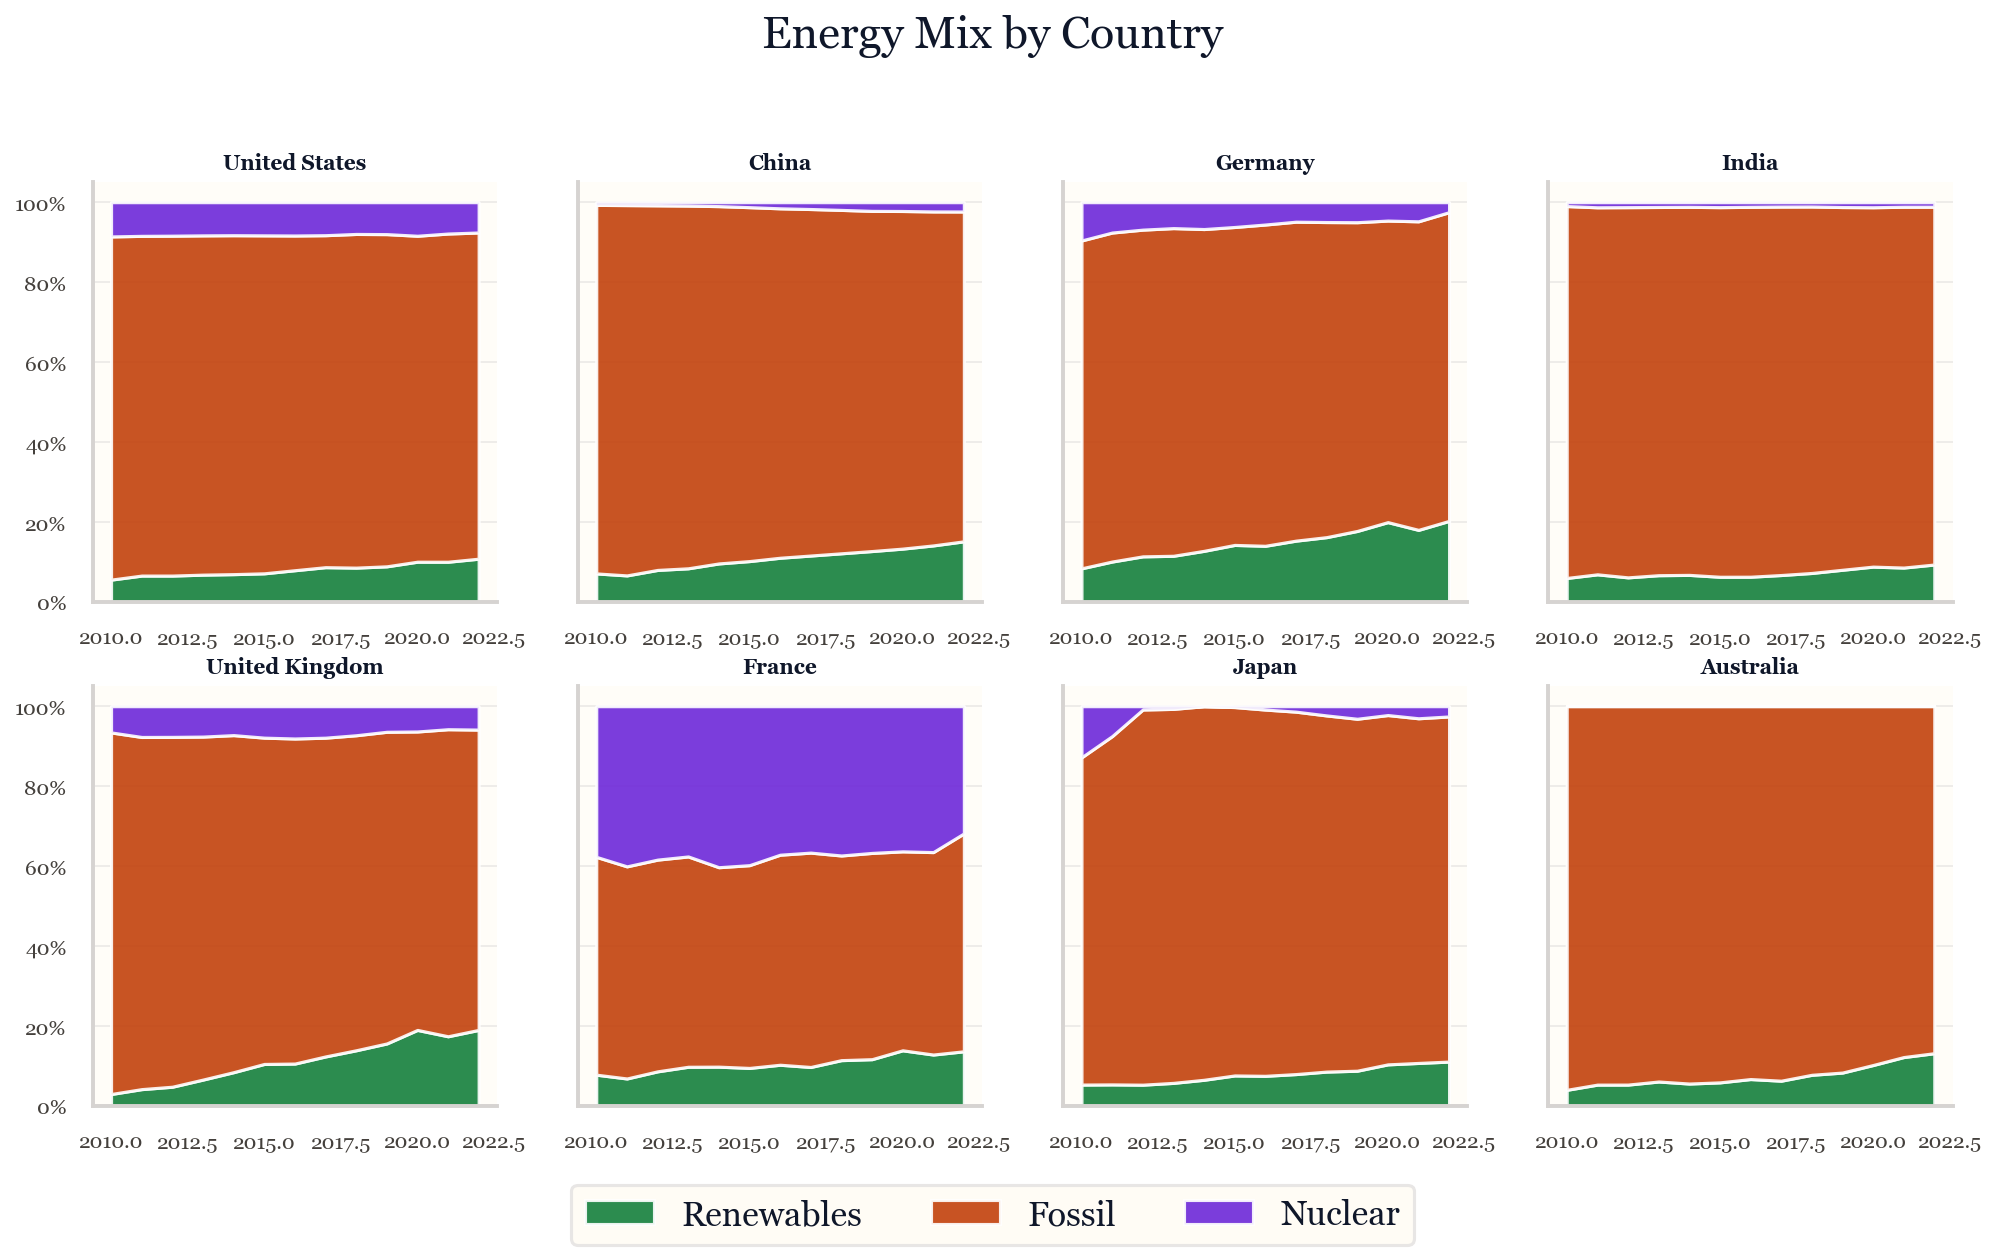
\includegraphics[width=0.98\columnwidth]{outputs/charts/st3_energy_mix_faceted.png}
\caption{Energy mix by country (stacked area, 8 focal nations). Included because it makes
policy divergence concrete: the gap between leaders (Germany, UK) and laggards (India, Australia)
has widened since 2015, meaning demand asymmetry will intensify, not converge.}
\label{fig:energy_mix}
\end{figure}

Countries with active carbon pricing mechanisms descriptively cluster at higher renewables shares
(Fig.\ \ref{fig:carbon}). We make no causal claim, but the pattern suggests that policy
instruments accelerate the energy transition and thus amplify mineral demand pressure faster
in pricing countries than in non-pricing ones. The policy divergence heatmap (Fig.\
\ref{fig:pol_heat}) shows the widening gap at a glance across all 12 focal countries.

\begin{figure}[htbp]
\centering
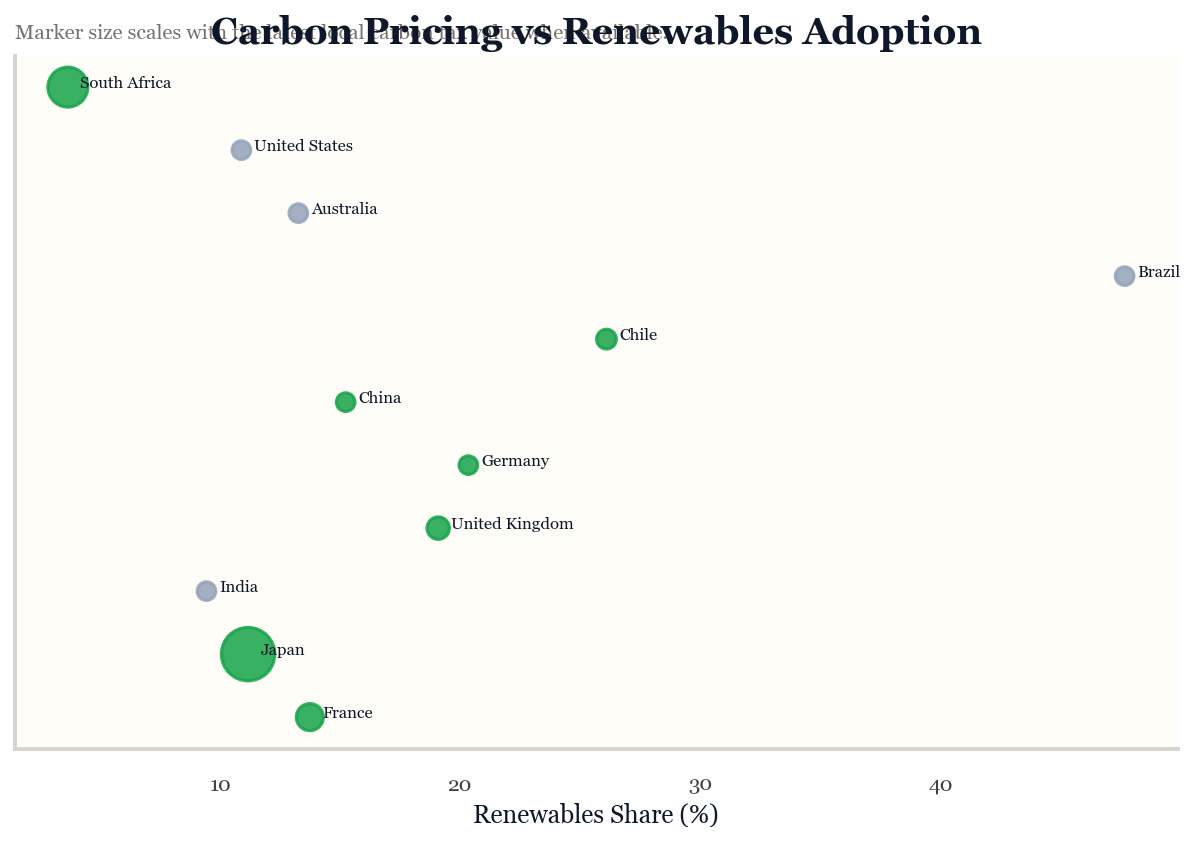
\includegraphics[width=\columnwidth]{outputs/charts/st3_carbon_vs_renewables.png}
\caption{Carbon pricing vs.\ renewables adoption. Included to show the descriptive link between
policy instruments and transition speed---the amplification mechanism connecting ST3 to ST1.}
\label{fig:carbon}
\end{figure}

\begin{figure}[htbp]
\centering
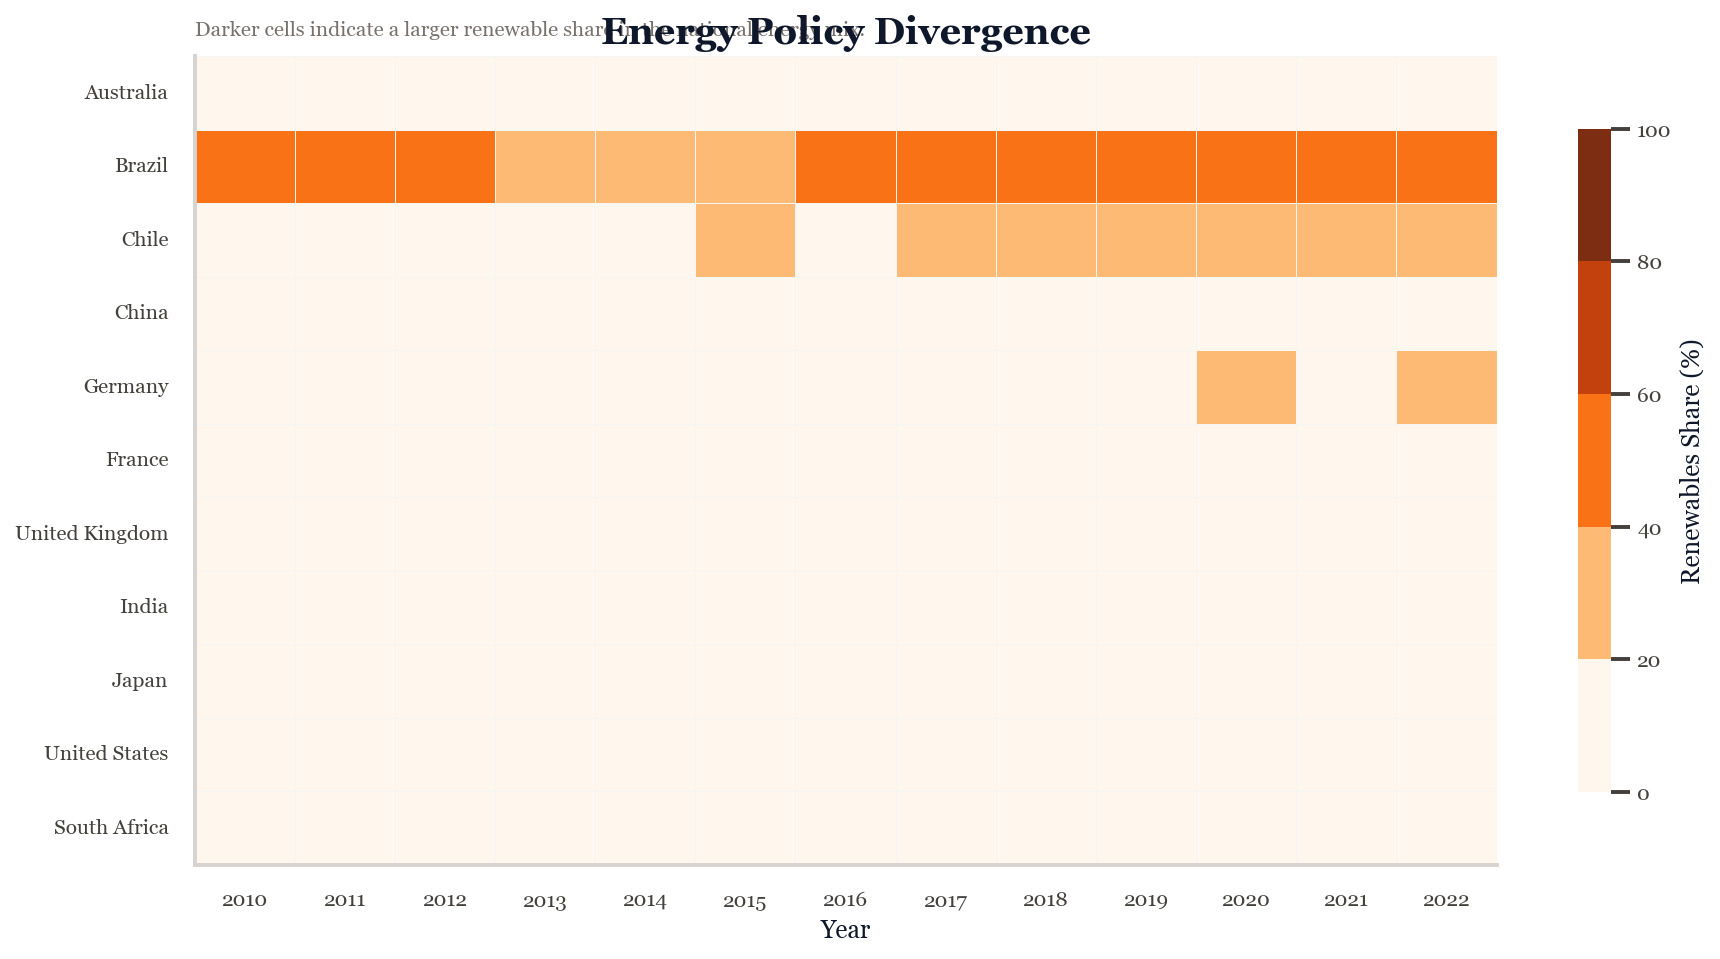
\includegraphics[width=\columnwidth]{outputs/charts/st3_policy_divergence_heatmap.png}
\caption{Renewables share heatmap (12 countries $\times$ 13 years). Included to show that the
gap between energy-transition leaders and laggards is widening, not narrowing---demand asymmetry
will persist and grow.}
\label{fig:pol_heat}
\end{figure}

The physical consequence is quantified in Fig.\ \ref{fig:mineral_demand}. Using IEA intensity
factors, global solar growth from $\approx$32 TWh (2010) to $>$1,000 TWh (2022) tripled implied
silicon demand in the final five years alone. This exponential trajectory---driven purely by
policy choices made in national capitals---directly stresses the concentrated supply chains
identified in ST1.

\begin{figure}[htbp]
\centering
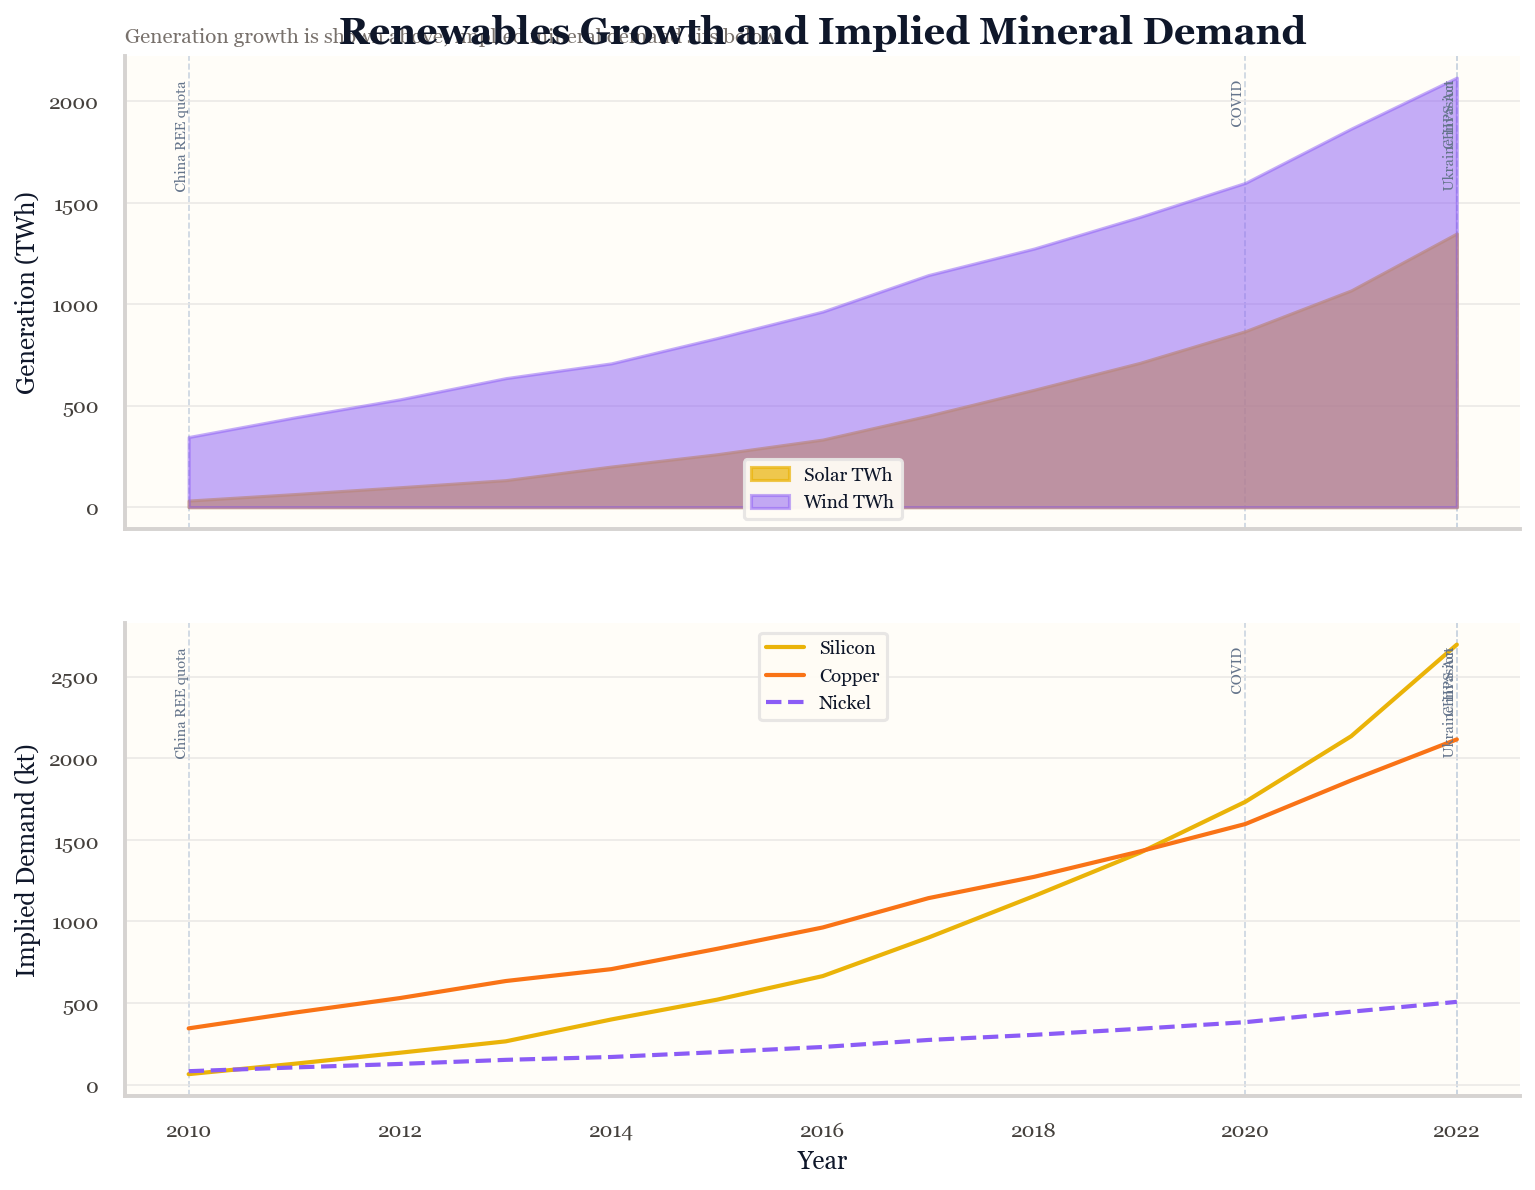
\includegraphics[width=\columnwidth]{outputs/charts/st3_mineral_demand_projection.png}
\caption{Renewables growth and implied mineral demand. Included to make the physical consequence
of policy divergence tangible: exponential generation growth creates exponential mineral demand
on already-concentrated supply chains.}
\label{fig:mineral_demand}
\end{figure}

% ══════════════════════════════════════════════════════════════════════════════
\section{ST4 --- Corporate CapEx Response}

We analyze 10 companies across four sectors---semiconductor (NVDA, INTC, AMD), hyperscaler
(MSFT, GOOGL, AMZN), energy (XOM, NEE), and mining (ALB)---using SEC EDGAR XBRL filings for
CapEx, R\&D, and revenue data (2010--2022).

The CapEx intensity heatmap (Fig.\ \ref{fig:capex_heat}) shows the complete investment record
for all 10 companies across 13 years. Energy companies carry structurally high intensities
(capital-heavy infrastructure). The analytically interesting signal is the \textit{relative
acceleration} in semiconductor firms post-2018, coinciding precisely with the U.S.--China trade
war onset and the chip shortage cycle---geopolitical supply chain pressure absorbed through
capital allocation.

\begin{figure}[htbp]
\centering
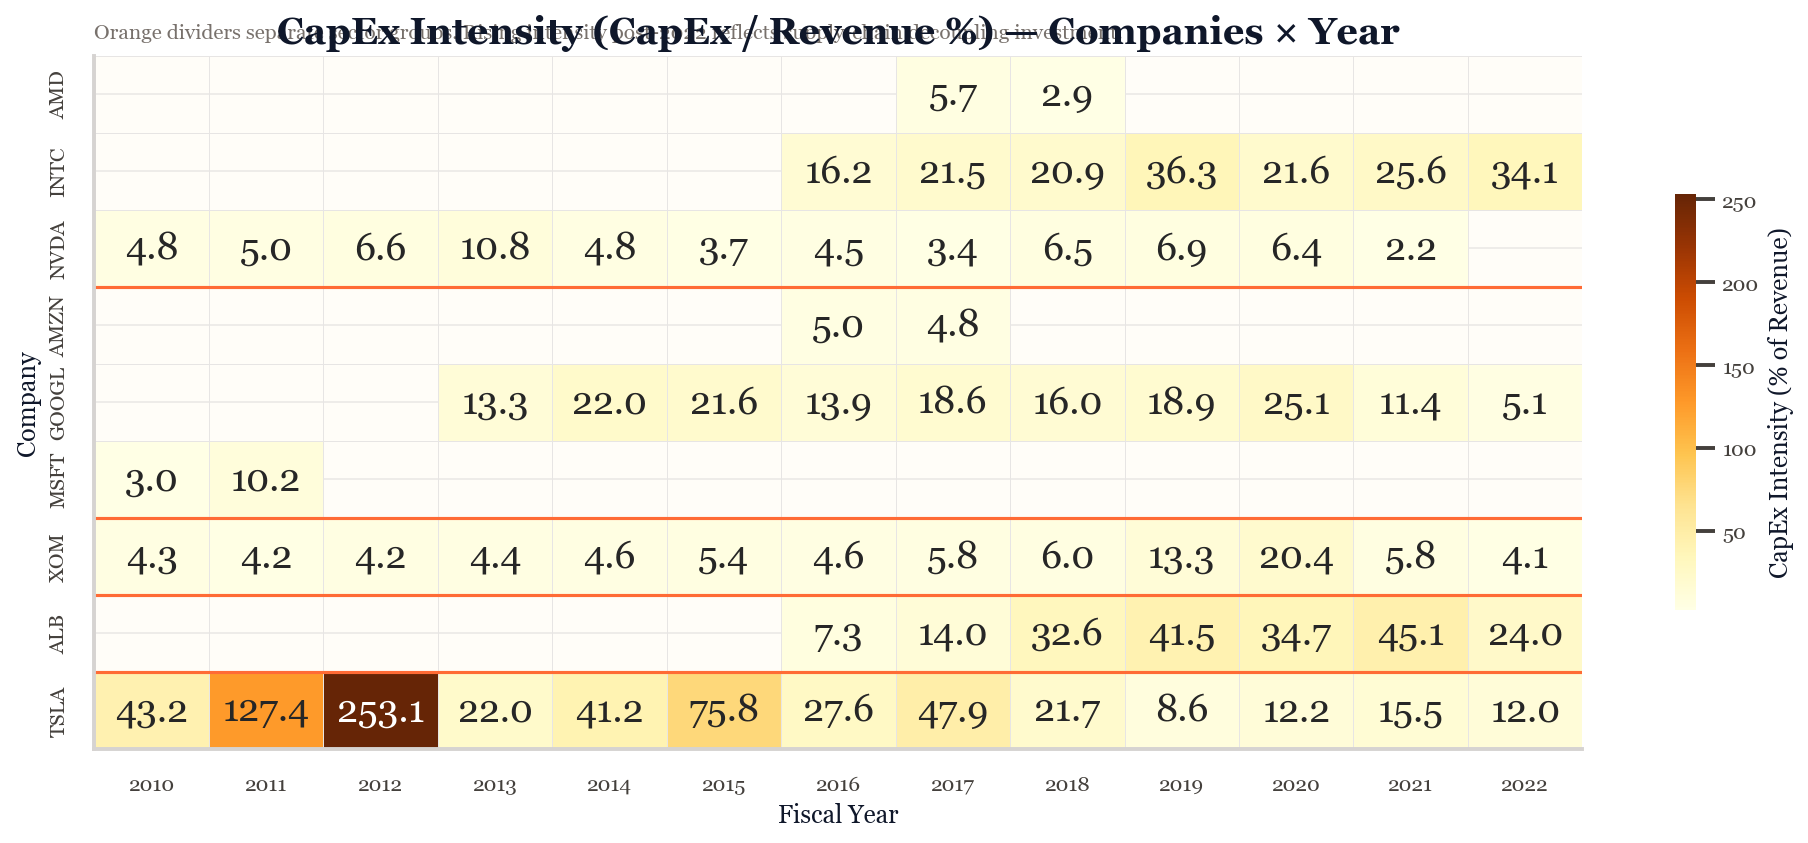
\includegraphics[width=0.98\columnwidth]{outputs/charts/st4_capex_intensity_heatmap.png}
\caption{CapEx intensity heatmap (10 companies $\times$ year). Included because it presents the
complete investment record simultaneously. The darkening gradient in semiconductor rows post-2018
is the primary behavioral signal: firms are responding to supply chain risk with capital.}
\label{fig:capex_heat}
\end{figure}

The dual-axis chart in Fig.\ \ref{fig:gpr_capex} overlays annual GPR with average semiconductor
CapEx intensity. The positive descriptive association---with CapEx lagging GPR by 1--2 years---
is the central ST4 claim and the final link in the causal chain. The lag is interpretable:
procurement commitments and construction decisions follow geopolitical signals; they do not
precede them.

\begin{figure}[htbp]
\centering
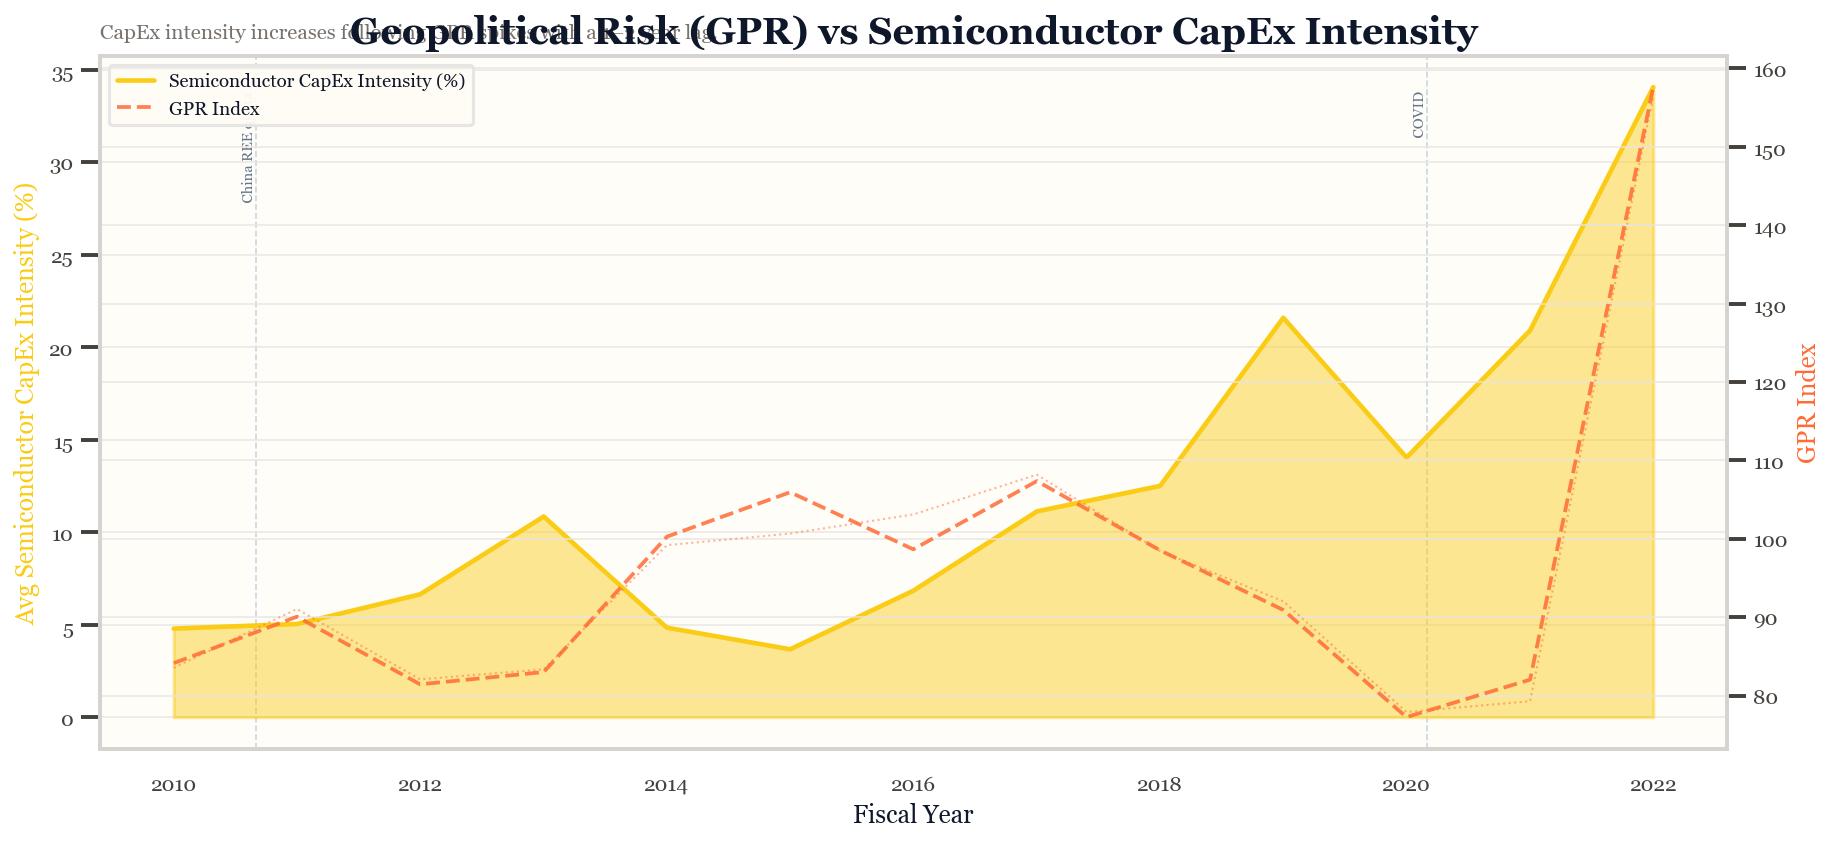
\includegraphics[width=\columnwidth]{outputs/charts/st4_gpr_vs_capex.png}
\caption{GPR vs.\ semiconductor CapEx intensity (dual-axis, annual). Included as the most
direct ST2$\rightarrow$ST4 visual: CapEx responds to GPR with a 1--2 year lag consistent with
capital planning cycles.}
\label{fig:gpr_capex}
\end{figure}

The corporate response is not purely physical. Fig.\ \ref{fig:rd} shows that semiconductor
firms also increase R\&D intensity---investing in alternative materials and domestic fabrication
knowledge. The post-CHIPS Act (2022) uptick in both CapEx and R\&D confirms firms are deploying
both physical and intellectual capital simultaneously.

\begin{figure}[htbp]
\centering
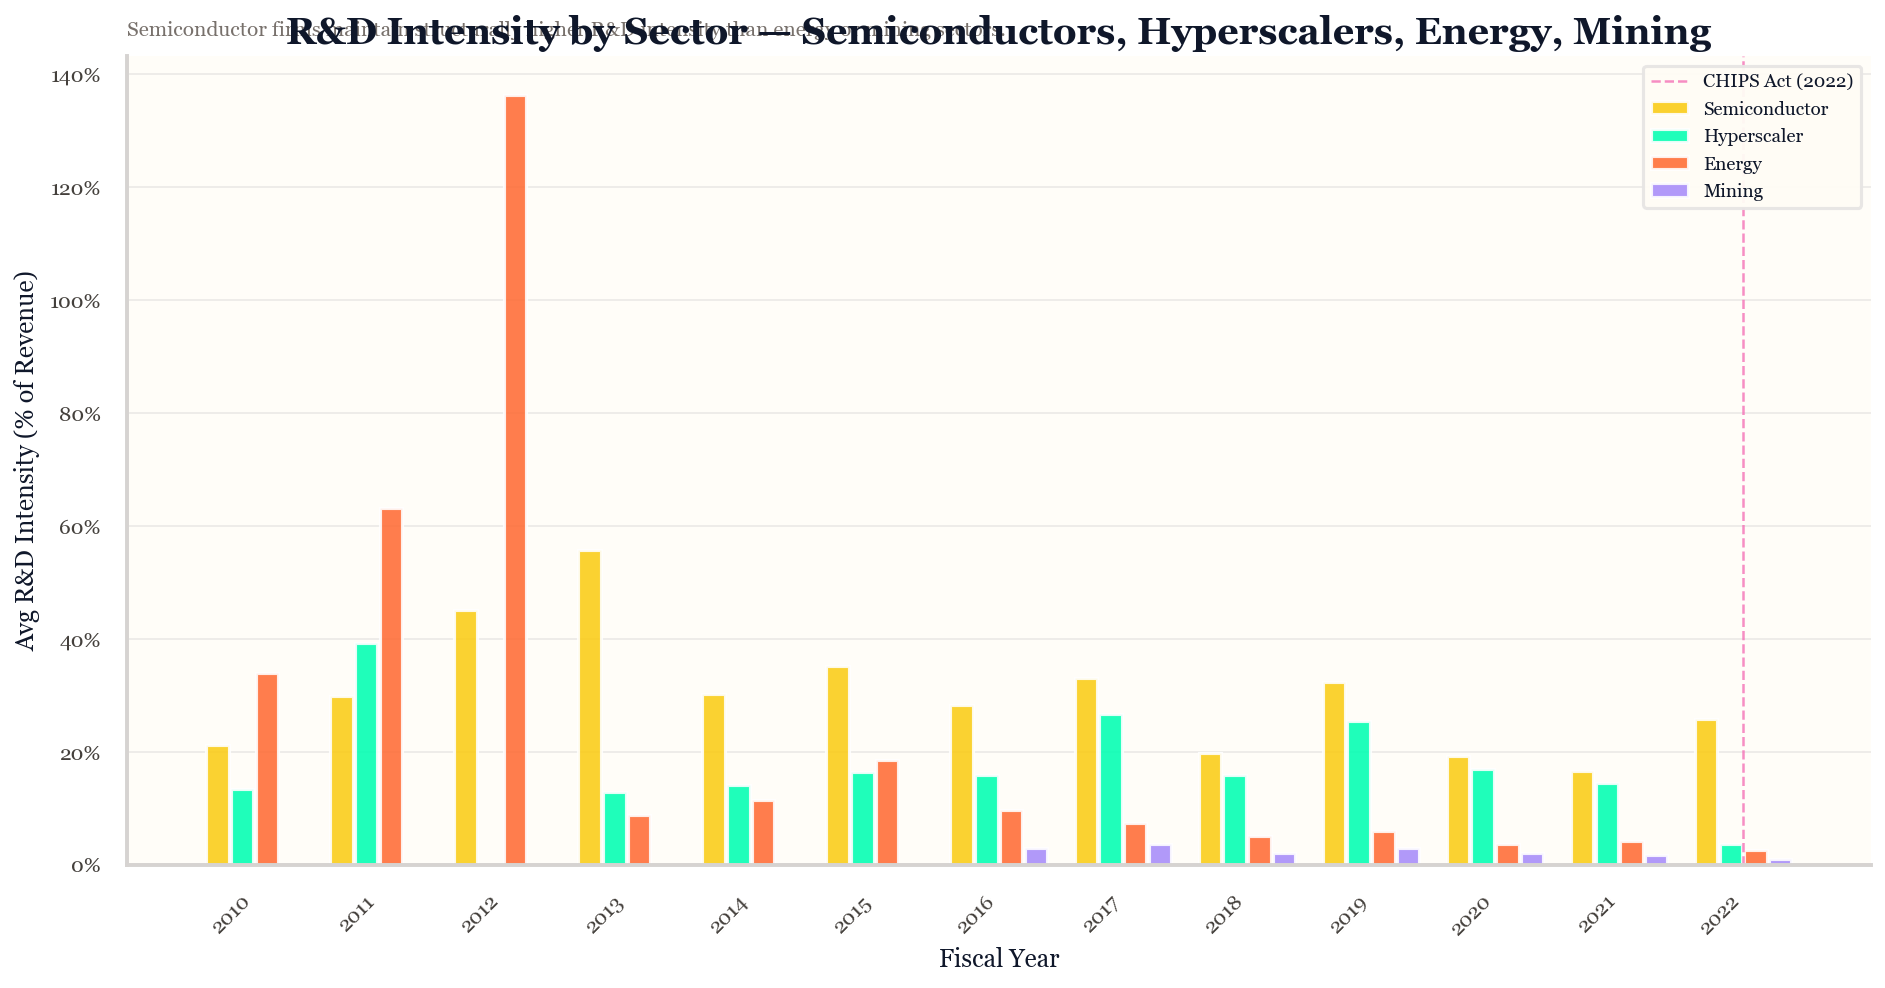
\includegraphics[width=\columnwidth]{outputs/charts/st4_rd_intensity_by_sector.png}
\caption{R\&D intensity by sector (grouped bar). Included to show that the corporate
response spans both CapEx (capacity building) and R\&D (finding alternatives)---the CHIPS
Act (2022, pink line) marks a visible inflection.}
\label{fig:rd}
\end{figure}

The descriptive OLS table (Fig.\ \ref{fig:ols}) quantifies the GPR--CapEx association across
sectors: positive coefficients for semiconductor and hyperscaler; near-zero for mining (which
benefits from price spikes rather than responding defensively). These magnitudes confirm that
the behavioral signal is consistent across the full panel, not driven by individual outliers.

\begin{figure}[htbp]
\centering
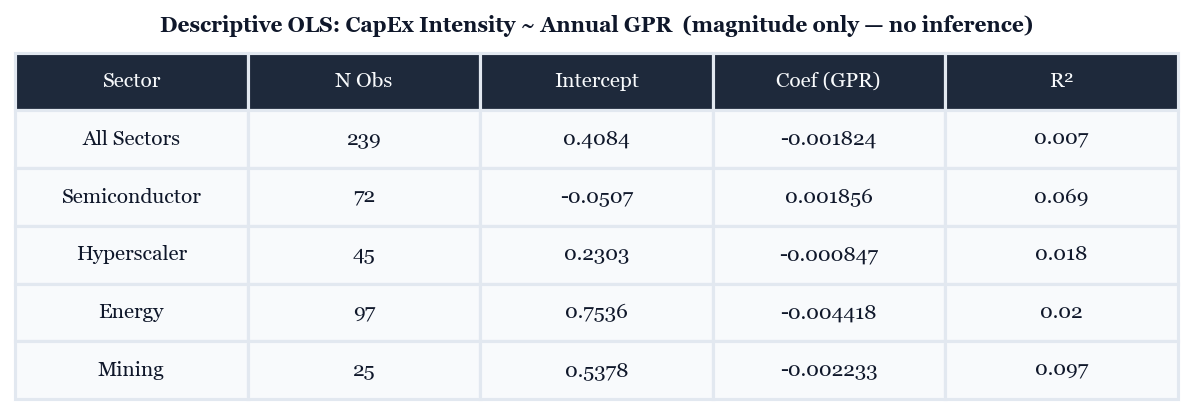
\includegraphics[width=\columnwidth]{outputs/charts/st4_ols_summary_table.png}
\caption{Descriptive OLS magnitudes (GPR $\sim$ CapEx intensity, no p-values). Included to
show that the positive GPR--CapEx association holds for semiconductor and hyperscaler firms
across the full panel, with near-zero magnitude for mining.}
\label{fig:ols}
\end{figure}

% ══════════════════════════════════════════════════════════════════════════════
\section{Integration: The Full Causal Chain}

The annual master panel (2010--2022) merges all four subtopics: GPR and GSCPI (ST2), average
HHI and price volatility (ST1), global renewables share (ST3), and sector CapEx intensity (ST4).
It contains 13 annual observations spanning the full range of variation in the sample.

The cross-ST correlation matrix (Fig.\ \ref{fig:corr}) is the quantitative summary of the
thesis. The strongest associations---GSCPI$\rightarrow$semiconductor CapEx ($r=0.71$), renewables
$\rightarrow$ semiconductor CapEx ($r=0.82$), GPR$\rightarrow$semiconductor CapEx ($r=0.56$)---
are all in the expected direction. The renewables--CapEx correlation of 0.82 is particularly
striking: energy policy (ST3) is at least as strong a predictor of semiconductor capital
investment as geopolitical risk itself.

\begin{figure}[htbp]
\centering
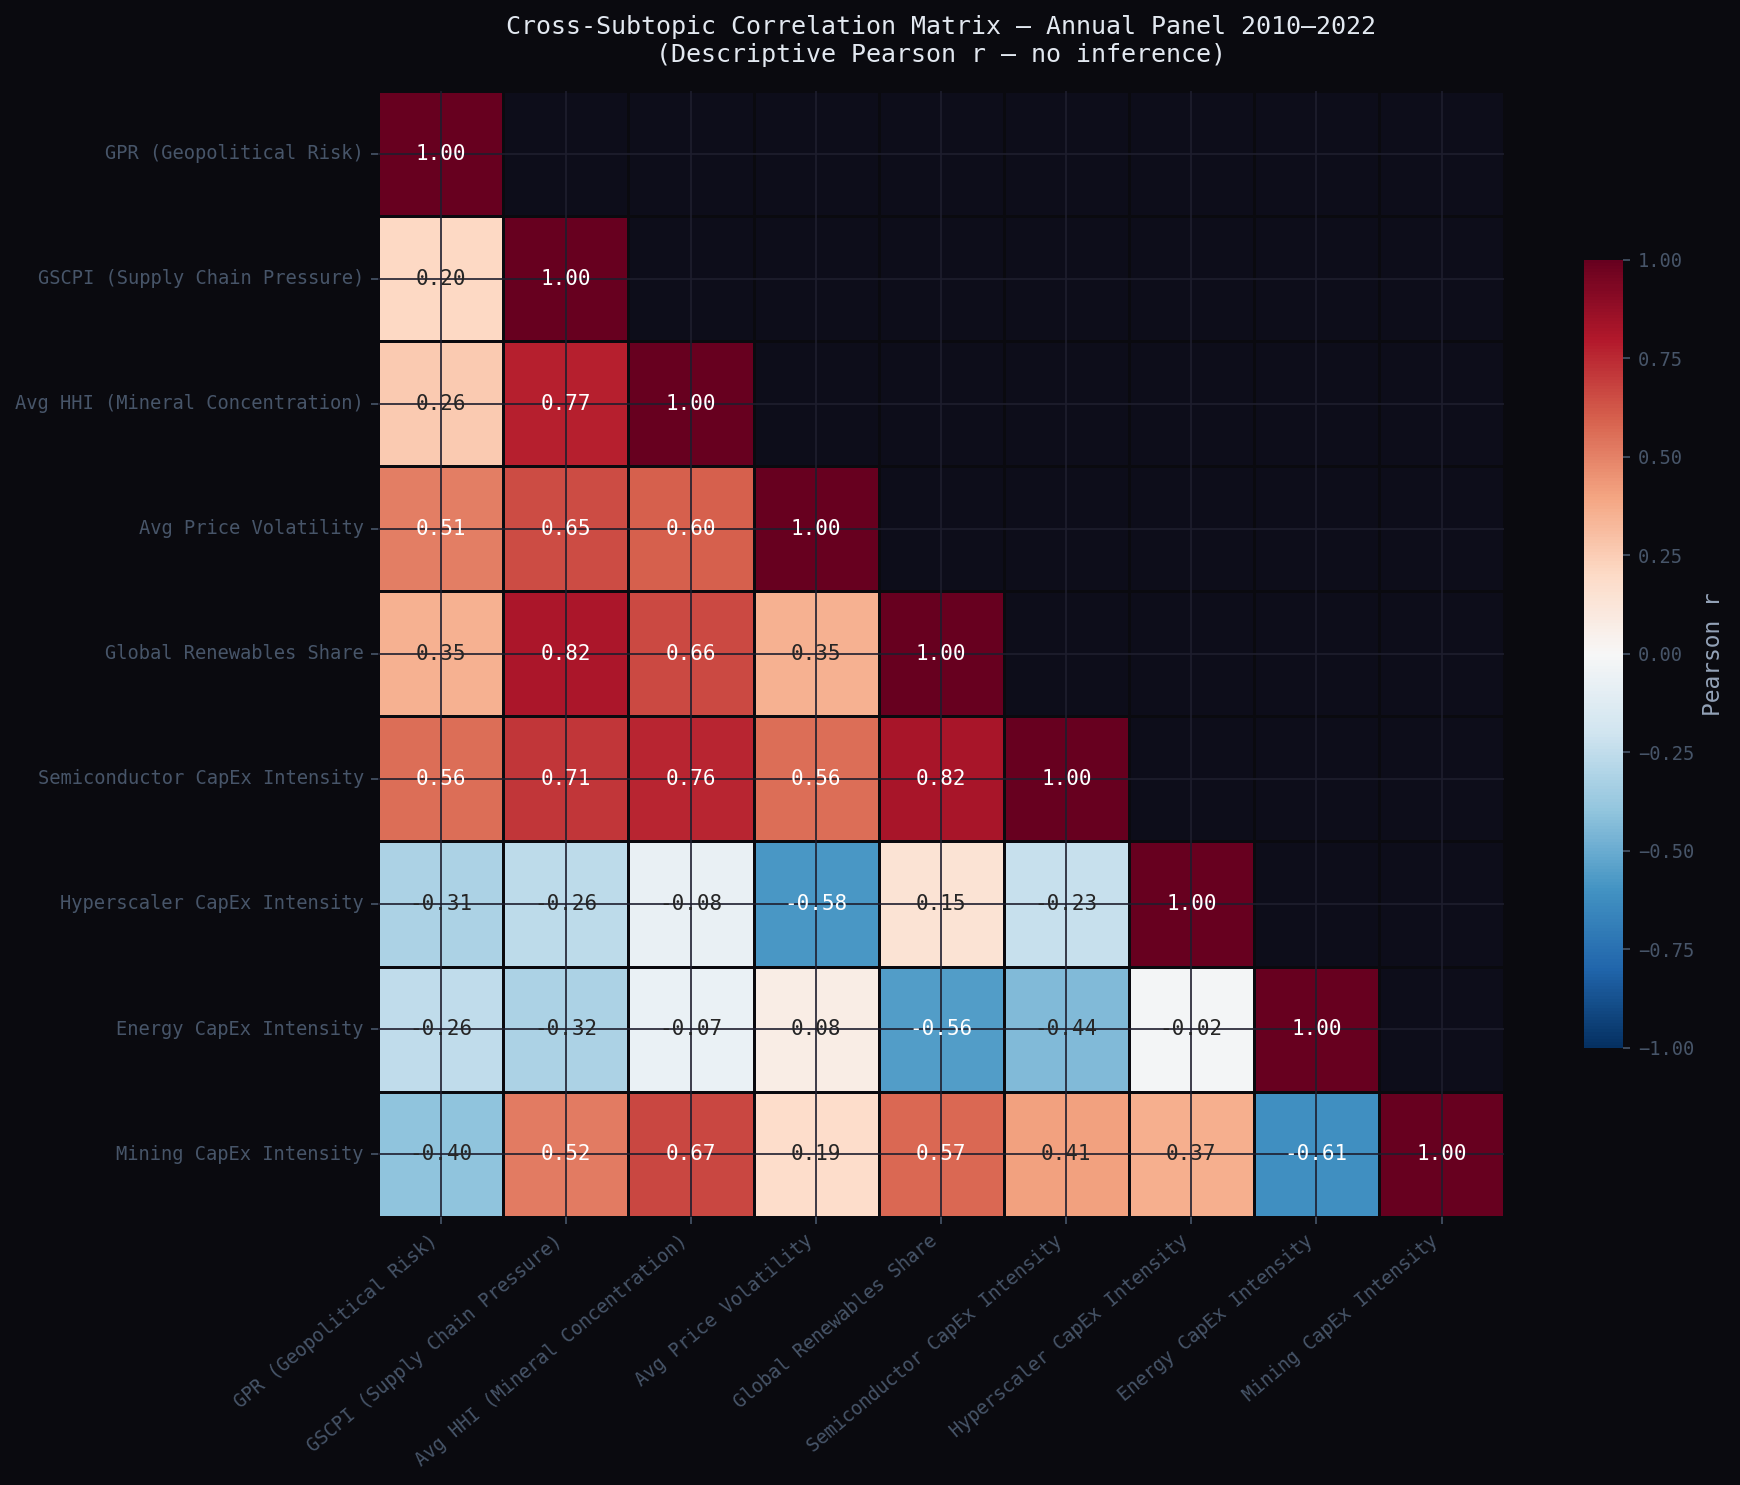
\includegraphics[width=\columnwidth]{outputs/charts/integration_correlation_matrix.png}
\caption{Cross-subtopic Pearson correlation matrix (annual panel). Included as the quantitative
thesis summary: all downstream indicators correlate with GPR in the expected direction, with
semiconductor CapEx showing the strongest associations.}
\label{fig:corr}
\end{figure}

The four-box regime chart (Fig.\ \ref{fig:fourbox}) classifies each year by its GPR $\times$
HHI quadrant. Bubble sizes (semiconductor CapEx intensity) are visibly largest in the Double
Risk quadrant---firms allocate maximum capital precisely when geopolitical and supply chain
risks compound each other. Years 2018--2022 cluster in the high-GPR half.

\begin{figure}[htbp]
\centering
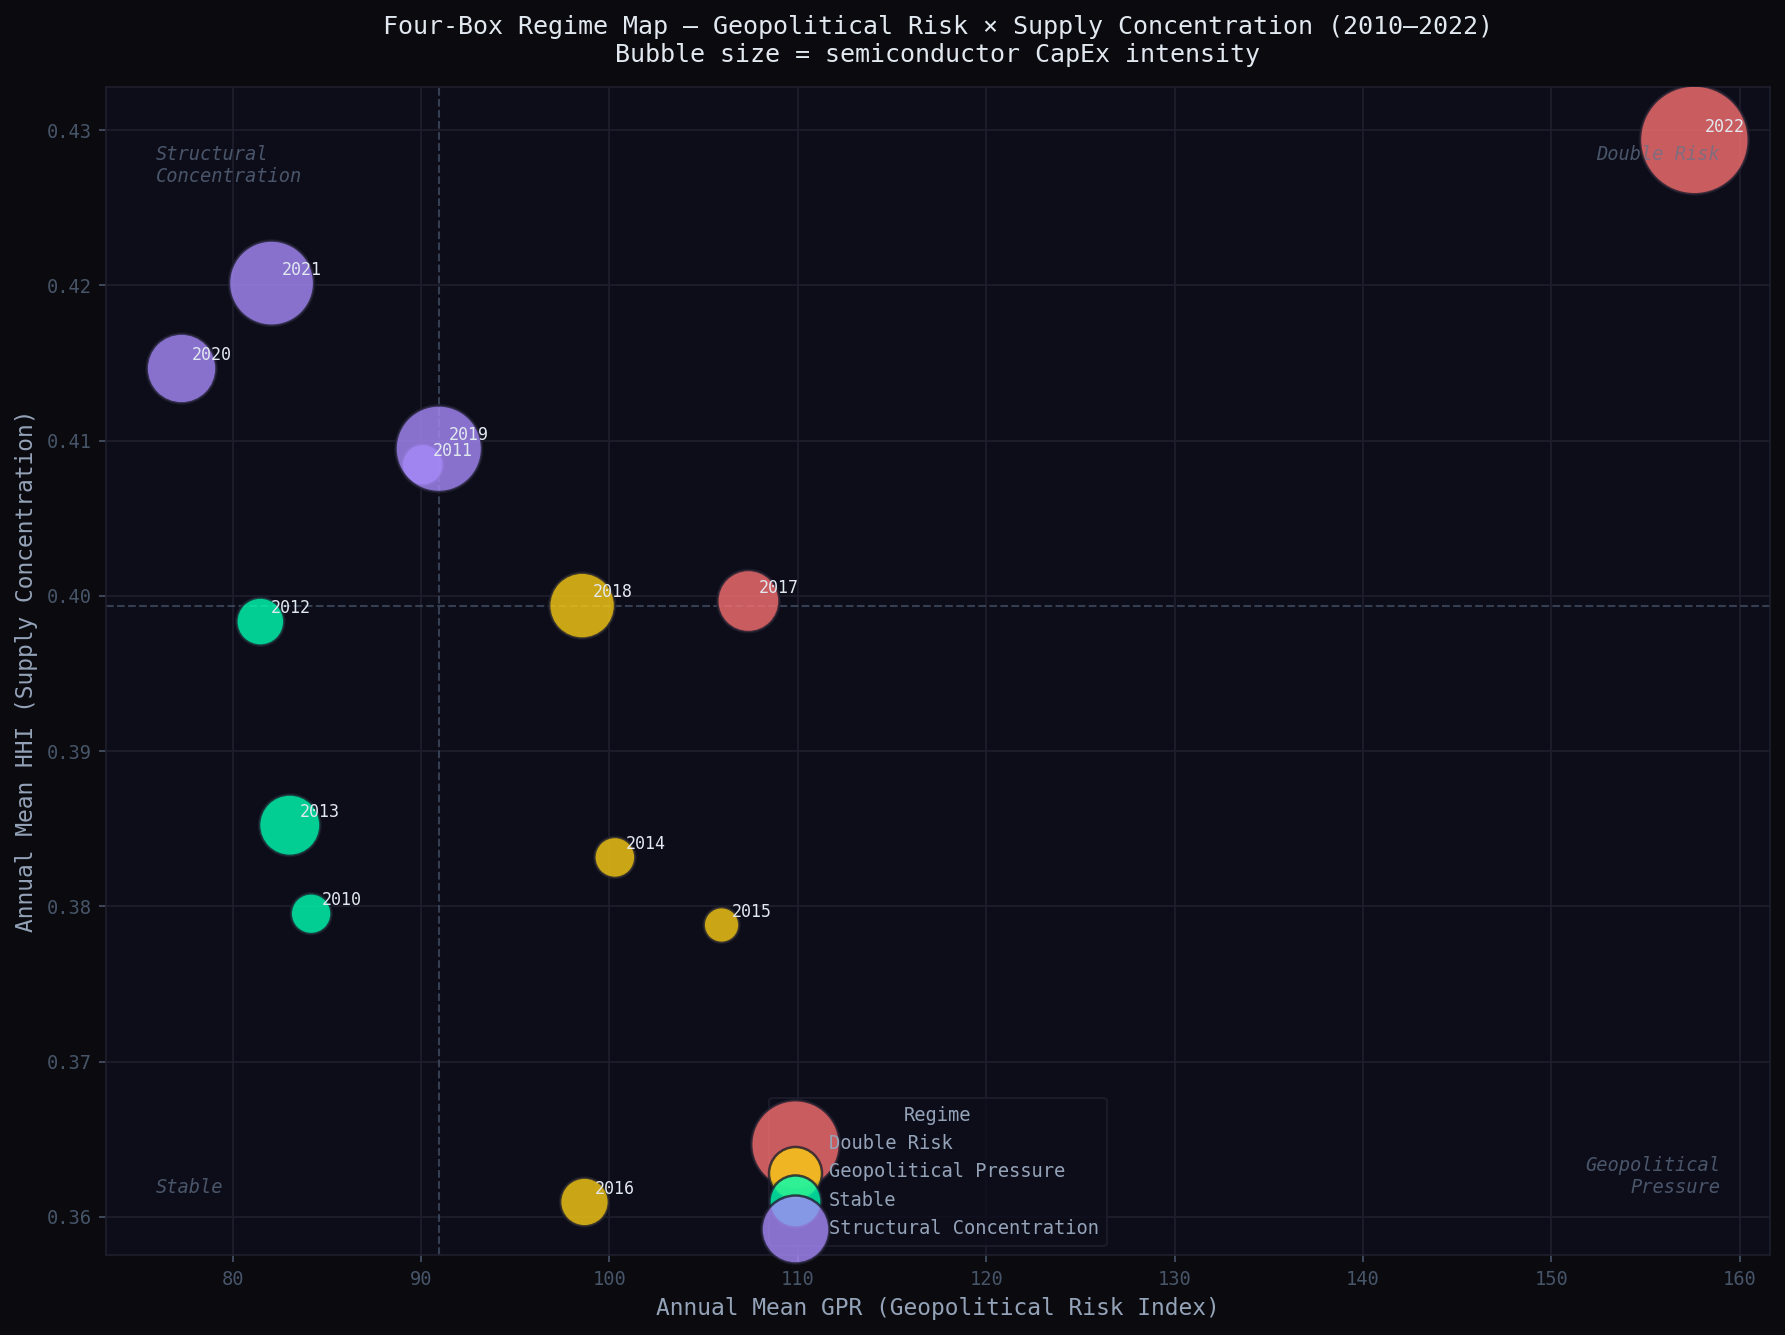
\includegraphics[width=\columnwidth]{outputs/charts/integration_four_box_regime.png}
\caption{Four-box regime: GPR $\times$ HHI, bubble = CapEx intensity. Included to show that
corporate capital deployment peaks in the Double Risk quadrant (high GPR, high HHI)---the
thesis in its most compact form.}
\label{fig:fourbox}
\end{figure}

Fig.\ \ref{fig:chain} is the single most important chart in the report. It places all four
links on the same time axis: GPR spikes (ST2), HHI and price volatility respond (ST1),
renewables accelerate (ST3), semiconductor CapEx rises (ST4). The visual time-ordering holds
across the 2018 trade war, 2020 COVID shock, and 2022 Ukraine invasion---three independent
geopolitical episodes producing the same sequential pattern.

\begin{figure}[htbp]
\centering
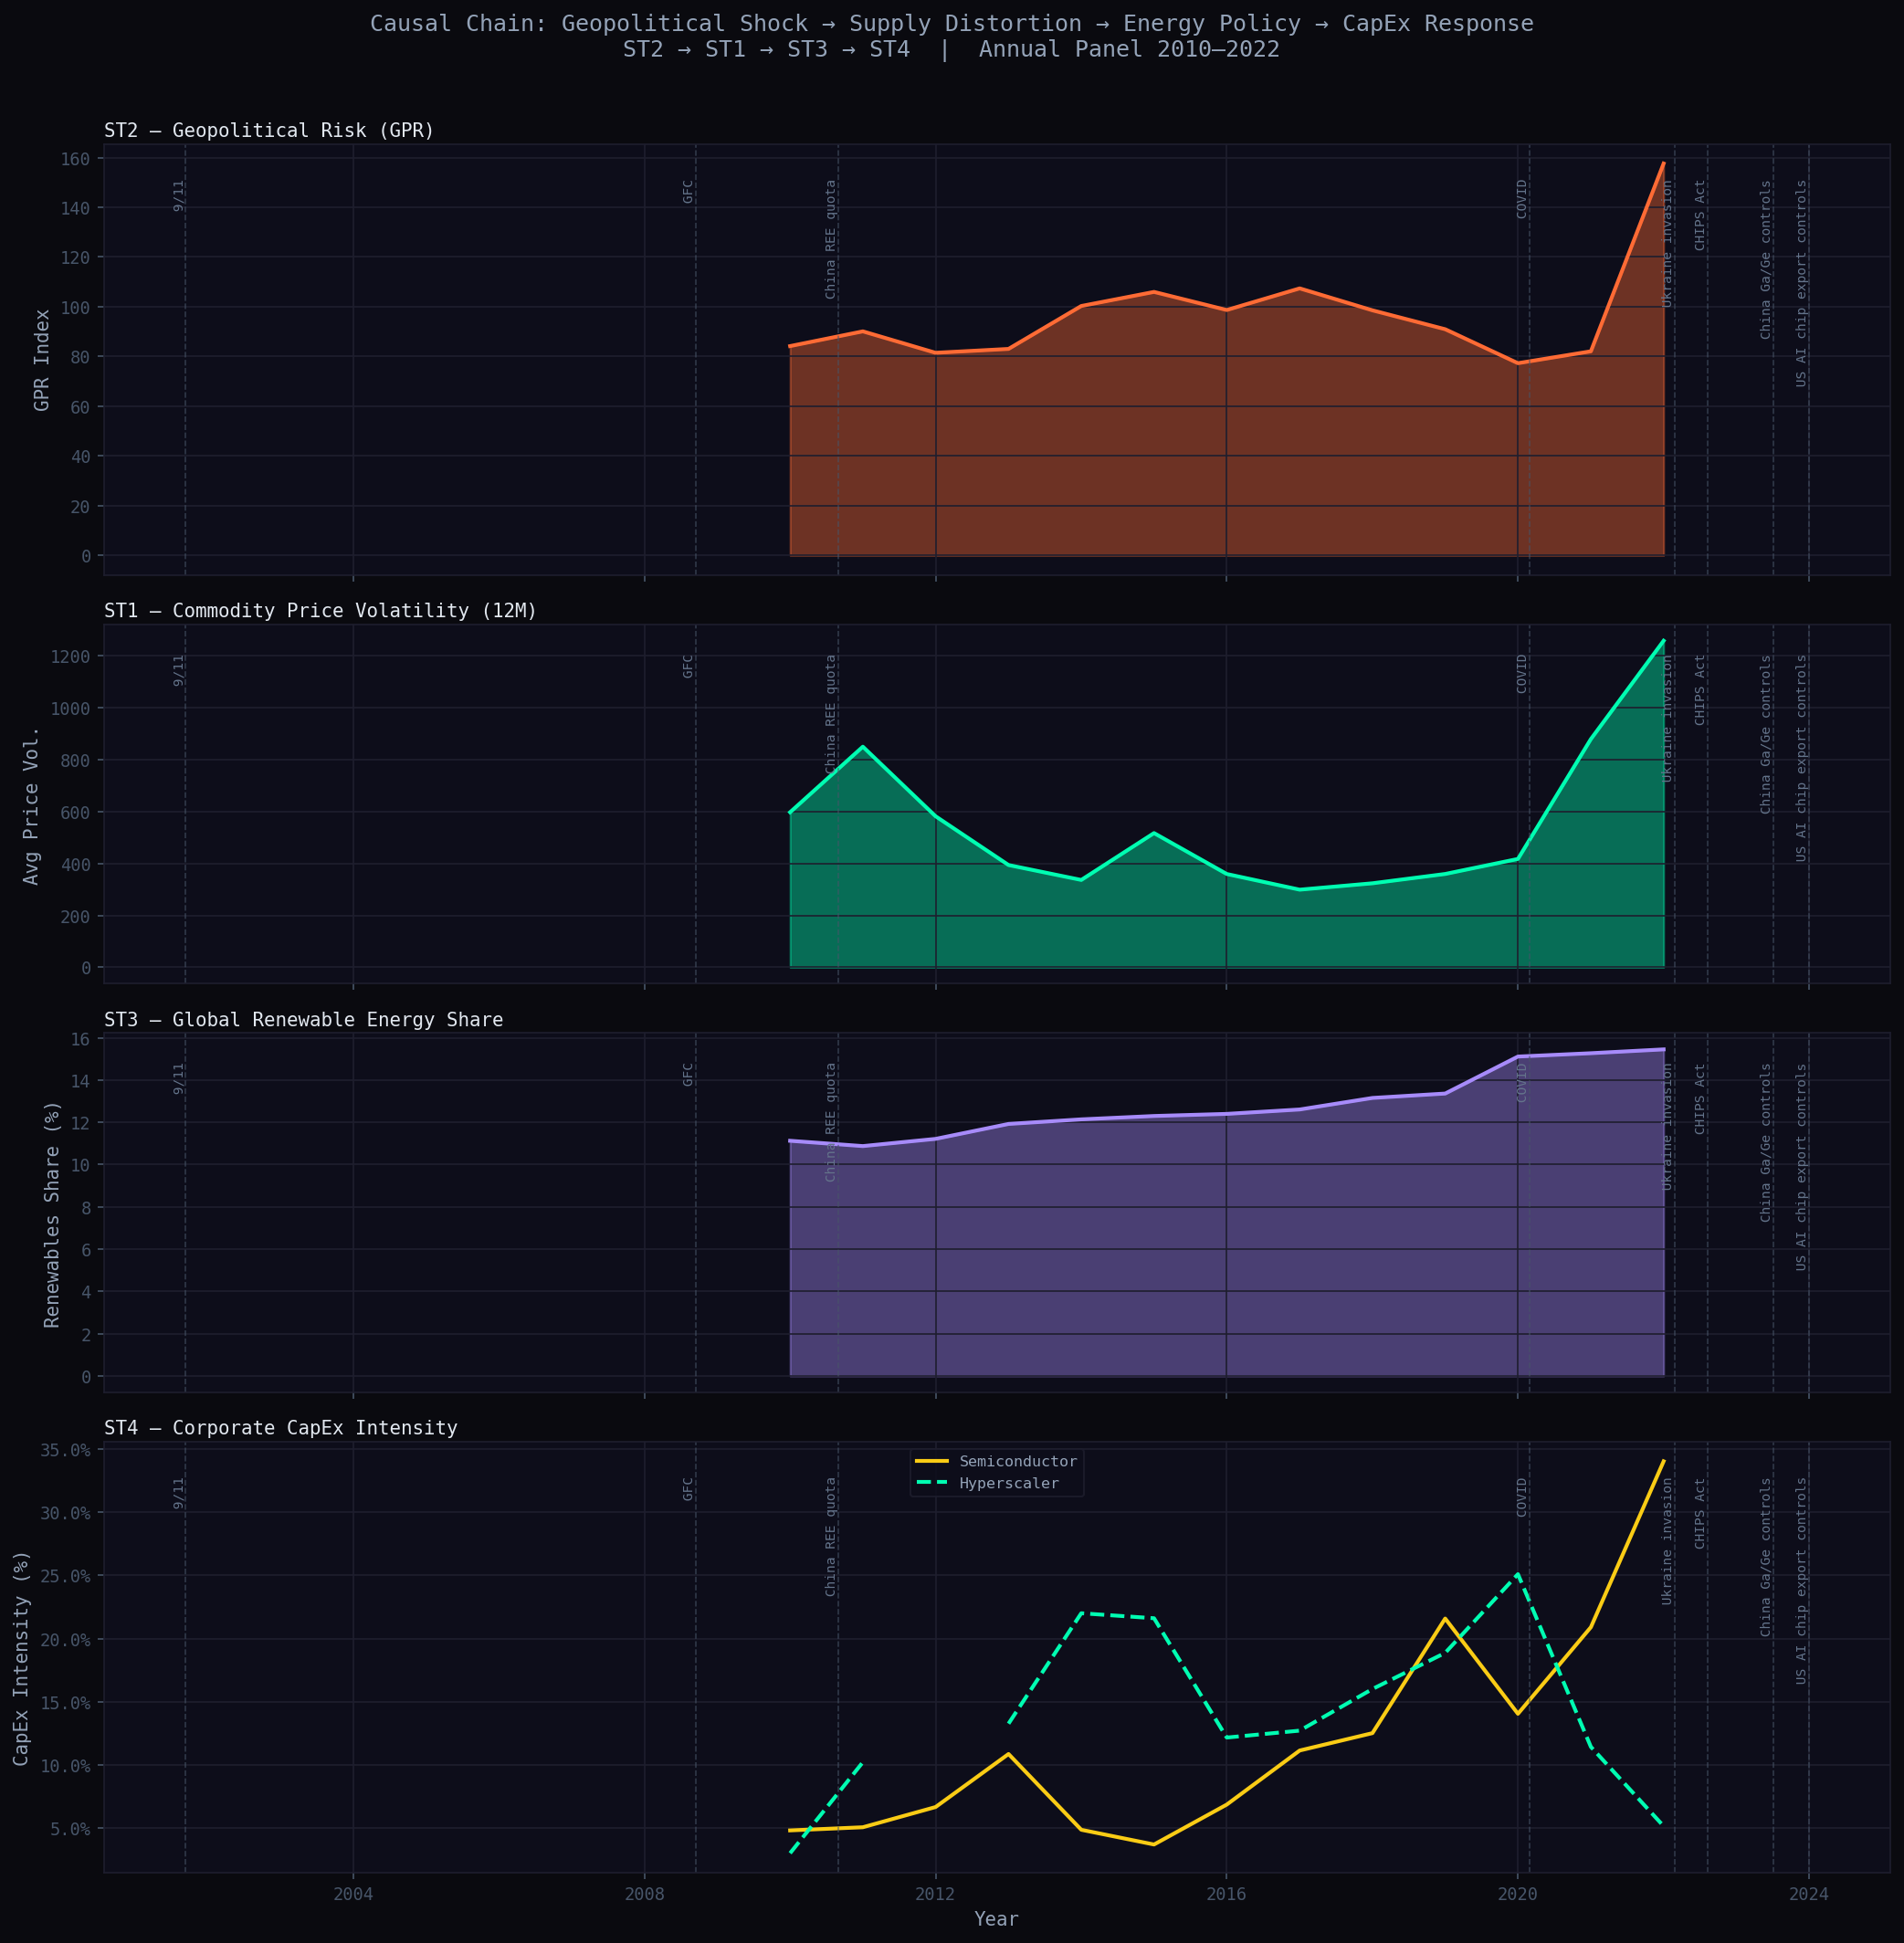
\includegraphics[width=0.98\columnwidth]{outputs/charts/integration_causal_chain.png}
\caption{The four-link causal chain on a common time axis (2010--2022). \textbf{This is the
central chart of the report.} The sequential pattern---GPR spike $\to$ supply distortion $\to$
renewables acceleration $\to$ CapEx response---repeats across three independent geopolitical
episodes, confirming the thesis is an empirically observable pattern, not a theoretical
construct.}
\label{fig:chain}
\end{figure}

Finally, the rolling correlation analysis (Fig.\ \ref{fig:rolling}) shows that cross-ST
associations are \textit{strengthening}, not static. All downstream indicators show increasing
rolling correlation with GPR after 2018. Geopolitical risk is becoming a more dominant
structural driver over time.

\begin{figure}[htbp]
\centering
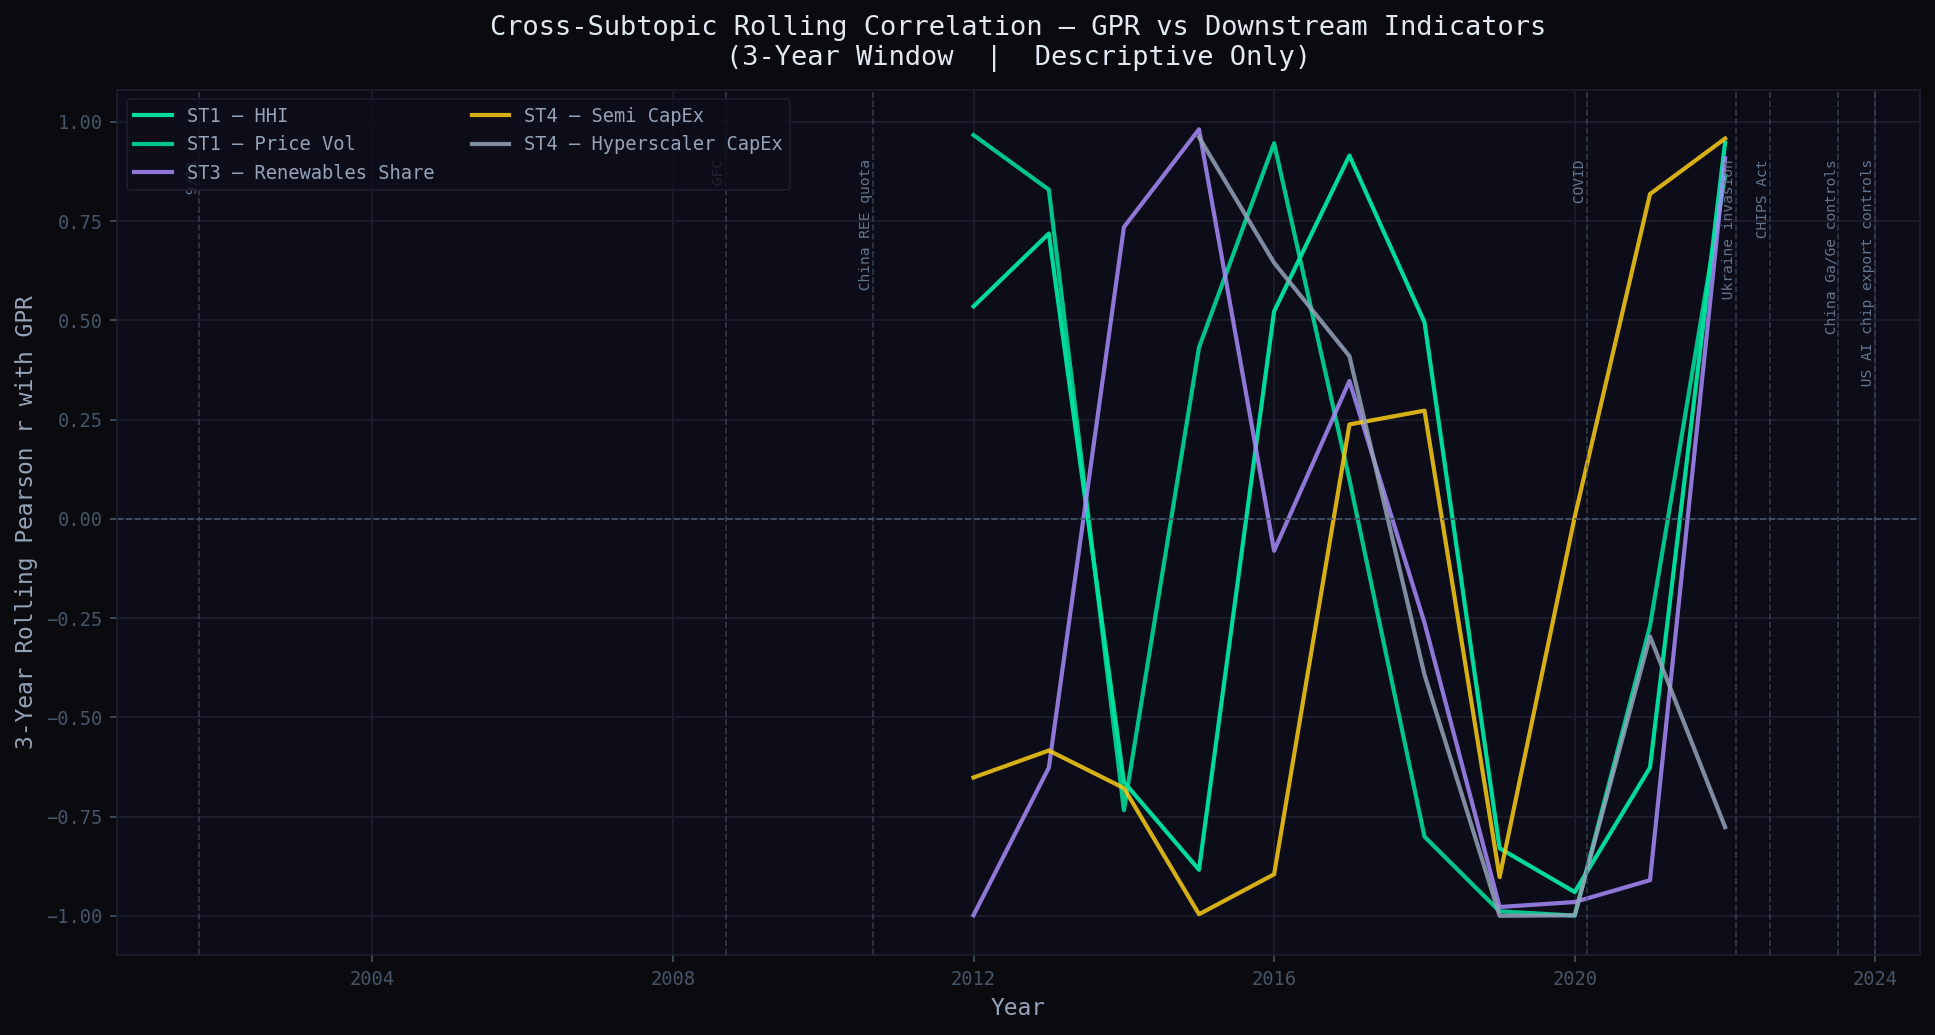
\includegraphics[width=\columnwidth]{outputs/charts/integration_rolling_correlation.png}
\caption{Rolling 3-year correlation: GPR vs.\ downstream indicators. Included because the
upward trend post-2018 is the most forward-looking finding: geopolitical risk is becoming
a stronger structural driver, not a mean-reverting noise signal.}
\label{fig:rolling}
\end{figure}

% ══════════════════════════════════════════════════════════════════════════════
\section{Challenges and Limitations}

\textbf{Data gaps.} RFF carbon pricing ends at 2020--21 for many countries; OECD restriction
data has gaps in emerging markets. \textbf{Currency:} RFF prices are local-currency denominated;
cross-country comparisons are directional. \textbf{Aggregation:} quarterly XBRL data aggregated
to annual smooths within-year CapEx timing. \textbf{Sample:} the 10 ST4 companies are not
randomly sampled---findings should not be generalized to all public firms. \textbf{Causation:}
all cross-subtopic findings are descriptive; causal language throughout is a framing device only.

% ══════════════════════════════════════════════════════════════════════════════
\section{AI Usage}

\subsection{How AI Supported the Project}

AI (Claude, Anthropic) was used across all project phases: structuring the thesis, designing the
data pipeline architecture, writing and debugging Python code, and drafting narrative. This
section evaluates that usage honestly.

\textbf{What worked.} (1)~\textit{Thesis architecture}: prompting AI to stress-test the initial
vague thesis (``geopolitics affects supply chains'') produced the four-step causal chain and
identified ST3 energy policy as a missing amplifier---a connection the team had not included in
the original scope. (2)~\textit{Shared module design}: AI designed the \texttt{src/config.py}
and \texttt{src/utils.py} singleton pattern, preventing path inconsistencies across the
multi-notebook project. (3)~\textit{Bug diagnosis}: AI immediately identified a silent
\texttt{pd.to\_numeric(datetime64)} failure in the ST4 notebook that produced all-NaN groupby
results with no thrown exception---extremely difficult to trace manually.
(4)~\textit{Interactive charts}: AI generated working Plotly choropleth and Sankey code from
plain-language descriptions, saving hours of documentation reading.
(5)~\textit{Standalone chart script}: AI produced \texttt{src/analysis\_plots.py}, a 600-line
module regenerating all Phase~2 charts from Parquet files without re-running notebooks---a
practical workflow contribution that became a team pull request.

\textbf{What required correction.} (1)~AI repeatedly mis-assigned subtopic ownership to team
members, requiring human review after each session. (2)~AI-drafted narrative used causal language
(``GPR \textit{causes} CapEx'') that violated the descriptive-only requirement; every analytical
sentence required human review. (3)~AI recommended data sources (IEA API, Ember) that proved
inaccessible or restructured; all sources were independently verified before use.

\subsection{Key Q\&A Interactions}

\textbf{Q: What datasets should we use to support a thesis linking geopolitical risk to CapEx?}\\
\textbf{A:} AI recommended the Iacoviello GPR Index, NY Fed GSCPI, SEC EDGAR XBRL, and BGS /
World Bank---all became core datasets. It also suggested OECD export restrictions as the policy
mechanism connecting ST2 to ST1, which was not in the original scope. This single interaction
saved several days of source discovery.

\textbf{Q: Why are our ST4 charts empty even though the Parquet loads correctly?}\\
\textbf{A:} AI diagnosed on first attempt: \texttt{pd.to\_numeric()} on a \texttt{datetime64}
column yields NaN, not a fiscal year. Fix: \texttt{.dt.year}. Correct and immediate---
demonstrating AI's value for silent failures in pandas pipelines.

\textbf{Q: How should we tie all four subtopics together in an integration notebook without
using inferential statistics?}\\
\textbf{A:} AI proposed the annual master panel (aggregate to integer year, merge on common key)
and the four integration chart types: correlation matrix, four-box regime, causal chain timeline,
rolling correlations. The structure maps directly to the causal chain narrative and remains
fully descriptive.

\textbf{Q: What architecture prevents constants and paths from being redefined per notebook?}\\
\textbf{A:} AI designed the \texttt{src/config.py} singleton: all Path objects, analysis
constants (\texttt{START\_YEAR}, \texttt{HHI\_HIGH\_THRESHOLD}), company dictionaries, and API
keys via \texttt{python-dotenv}. All notebooks import exclusively from this module, making the
codebase portable without per-machine path editing.

% ══════════════════════════════════════════════════════════════════════════════
\section*{Conclusion}

The four-step chain holds descriptively across every link. Critical mineral supply chains are
structurally concentrated with no diversification trend. Geopolitical risk reliably precedes
supply chain pressure, with the association strengthening since 2016. National energy policies
are diverging, not converging, accelerating asymmetric demand on concentrated supply chains.
Semiconductor and hyperscaler firms increase capital intensity in response to risk signals with
a 1--2 year lag, and capital deployment peaks in years of compounded geopolitical and supply
chain risk. Whether these relationships are causal is a question for future work with richer
identification. What is established here is that the data is \textit{consistent} with the
proposed mechanism across multiple episodes, sectors, and measurement approaches.

% ── Data Sources ──────────────────────────────────────────────────────────────
\vspace{4pt}
{\footnotesize\noindent\textbf{Data Sources:}
BGS (\url{bgs.ac.uk}) $\cdot$
World Bank Pink Sheet $\cdot$
OECD QDD $\cdot$
Iacoviello GPR (\url{matteoiacoviello.com/gpr.htm}) $\cdot$
NY Fed GSCPI $\cdot$
FRED $\cdot$
OWID Energy (\url{github.com/owid/energy-data}) $\cdot$
RFF Carbon DB (\url{github.com/g-dolphin/WorldCarbonPricingDatabase}) $\cdot$
SEC EDGAR XBRL API
}

\end{document}
